\documentclass{article}
\usepackage[utf8]{inputenc}
\usepackage{amsmath}
\usepackage{amssymb}
\usepackage{enumerate}
\usepackage{adjustbox}
\usepackage{pdflscape}
\usepackage{multirow}
\usepackage{float}
\usepackage[section]{placeins}
\usepackage{booktabs}
\usepackage{array}
\usepackage{xurl}
\usepackage{xr}
\externaldocument[main-]{main}
\emergencystretch=1em
\usepackage[numbers]{natbib}
\usepackage{hyperref}
\newif\ifdraftnotes
\draftnotesfalse
\ifdraftnotes
  \usepackage{todonotes}
\else
  \usepackage[disable]{todonotes}
\fi
\usepackage{graphicx}
\usepackage{tikz}
\usetikzlibrary{arrows.meta,positioning,shapes.geometric}
\graphicspath{{fig/}}
\hypersetup{
    colorlinks=true,
    linkcolor=blue,
    urlcolor=blue,
}
\newcommand{\method}{LinkGDA}
\newcommand{\projection}{OWL2Vec*}
\newcommand{\projectionextended}{GDAProjector}
\newcommand{\std}[1]{{\scriptsize $\pm$#1}}
\newcommand{\f}[1]{\textbf{#1}}
\newcommand{\s}[1]{\underline{#1}}
\newcommand{\revdone}[1]{\todo[inline,color=green!20,size=\footnotesize]{\textbf{REVIEW (applied):} #1}}
\newcommand{\revtodo}[1]{\todo[inline,color=orange!25,size=\footnotesize]{\textbf{REVIEW (action needed):} #1}}
\title{PhenoQuery: phenotype-query learning and evaluation biases in gene--disease association prediction\\ Supplementary Material}
\author{Fernando Zhapa-Camacho \and Naeema Muhammed \and Robert Hoehndorf}
\date{}
\renewcommand{\thetable}{S\arabic{table}}
\renewcommand{\thefigure}{S\arabic{figure}}
\begin{document}
\maketitle

\section{Data and computational provenance}

The computational inputs are retained prepared gene--phenotype, disease--phenotype,
gene--function, gene--expression and gene--disease tables, together with pinned
OWL ontologies. The tables were recovered from the study's original data
checkout. Source metadata identifies HPO v2026-01-08, UPheno v2025-10-12,
GO annotations from 2025-12-04, GTEx E-GTEX-8 and the MGI phenotype and human
orthology reports. Some original provider files remain unavailable, so exact
reproduction starts from the retained prepared tables. File identities and
processing commands are documented in the machine-readable manifests.

The preparation code assigns each MGI genotype phenotype to every listed
marker with a mapped human ortholog, including multi-marker genotypes. GO
annotations include biological process, molecular function and cellular
component terms from all evidence codes, excluding NOT-qualified annotations.
The gene--disease loader retains every association type in the source table
before the benchmark's coverage and disease filters. GTEx expression requires
TPM greater than 4; case-insensitive matching to primary UBERON labels retains
51 of 53 tissues, excluding hippocampus and skin. The reported source access
dates are MGI phenotypes 2026-02-05, orthology 2026-02-08, GTEx 2026-02-08,
UniProt mapping 2026-01-29 and Ensembl mapping 2026-02-10; these dates derive
from the study metadata. Graph and semantic-similarity queries retain only
UPheno-represented terms, dropping 16,124 of 164,006 prepared disease--phenotype
rows. Phive receives all supplied HP terms, including onset and inheritance,
through its native query interface.

GO annotations map UniProt accessions to Entrez genes. Fields containing
multiple positive-integer Entrez identifiers are split and deduplicated. This
produces 317,868 gene--function pairs for 18,904 genes; 299 annotation rows
have terms outside the retained graph, while every gene retains a represented
function. Of 13,626 genes with prepared MGI phenotype annotations, 13,625 have
at least one phenotype represented in UPheno. The latter set defines the main
candidate pool independently of disease-association labels.

The disease-association source has 15,782 pairs. Filtering for represented
phenotypes on both the gene and disease yields 6,571 main-benchmark pairs.
Among 1,366 pairs whose genes lack MGI phenotypes, requiring GO annotations
and disease HPO profiles leaves 559; removing main-benchmark diseases leaves
499; excluding phenotype-set Jaccard similarity of at least 0.5 to a
main-benchmark disease leaves 425 pairs from 364 genes and 417 diseases.
The primary pool comprises all 5,696 GO-annotated genes without MGI phenotypes.
The secondary pool comprises all 18,904 GO-annotated genes.

We project UPheno, GO and UBERON independently with mOWL v1.0.3 and its
OWL2VecStar projector, enabling bidirectional taxonomy and excluding literals.
The pinned OWL versions are UPheno v2025-10-12, GO 2026-01-23 and UBERON
2025-12-04. Each projection runs in a fresh process; we deduplicate final
triples. The historical KGE environment uses Python v3.11.15 and Java 17, with its
package resolution retained in the Pixi manifest and lockfile. The controlled
query campaign uses a separately archived Python 3.10.22 environment with
PyTorch 2.1.2+cu121 and PyG 2.4.0; its 70 Conda package identities and 43
Python distributions were reproduced from the published locks. GPU training and ULTRA inference ran on ORIX; semantic similarity
and Phive ran through IBEX Slurm. Submission scripts retain resource requests,
seeds and complete command lines.

Every score matrix has an ordered candidate sidecar. The audit checks score
width, true-gene index, duplicate association rows, finite values, and identical
score vectors for repeated diseases. Fold aggregation checks candidate hashes
and disjoint test diseases. Fixed-reference checks require distinct training
diseases, population standard deviations, matching candidate order and exclusion
of test diseases. Per-association ranks, both pair- and disease-averaged metrics,
filtered sensitivities and candidate-percentile endpoints are retained as JSON.
The prepared-input release at
\url{https://github.com/bio-ontology-research-group/link-gda/releases/tag/inputs-20261028-v1}
contains 35 checksum-bound archives. A fresh public download verified all 469
files; the ten benchmark caches, ten matched graphs and 50 PhenoQuery graphs
were also reconstructed byte-for-byte. Prediction and trained-checkpoint
archives are separate deliverables and remain under verification.

\begin{table}[htbp]
  \centering
  \caption{Data sources and prepared input counts before graph-term coverage filtering.
    Gene--disease pairs require non-empty represented phenotype profiles for both entities.}
  \label{tab:datasets}
  \small
  \begin{tabular}{llr}
    \toprule
    Relation & Source file & \# pairs \\
    \midrule
    Gene--Phenotype          & \texttt{MGI\_GenePheno.rpt}    & 213{,}988 \\
    Disease--Phenotype       & \texttt{phenotype.hpoa}        & 164{,}006 \\
    Gene--Function           & \texttt{goa\_human.gaf.gz}     & 317{,}868 \\
    Gene--Expression site    & \texttt{tpmss.tsv} (E-GTEX-8)  & 536{,}923 \\
    Gene--Disease (total)    & \texttt{genes\_to\_disease.txt} & 6{,}571 \\
    \bottomrule
  \end{tabular}
\end{table}


\begin{figure*}[t]
\centering
\begin{minipage}[t]{0.52\textwidth}
\vspace{0pt}
{\small\bfseries (a) Training graph}\par\smallskip
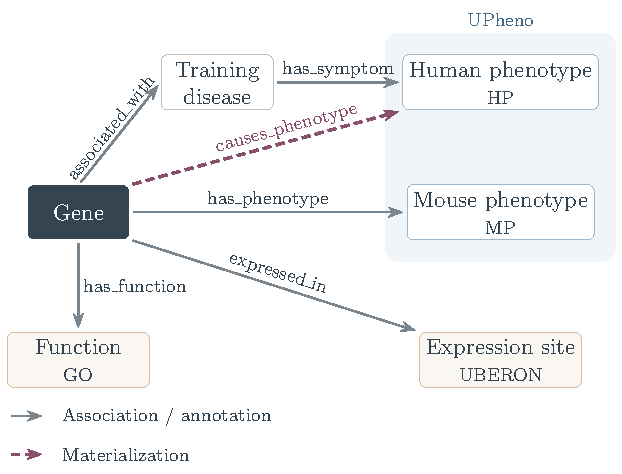
\includegraphics[width=\linewidth]{fig/overview_graph_clean.pdf}
\end{minipage}\hfill
\begin{minipage}[t]{0.44\textwidth}
\vspace{0pt}
{\small\bfseries (b) Per-gene calibration}\par\smallskip
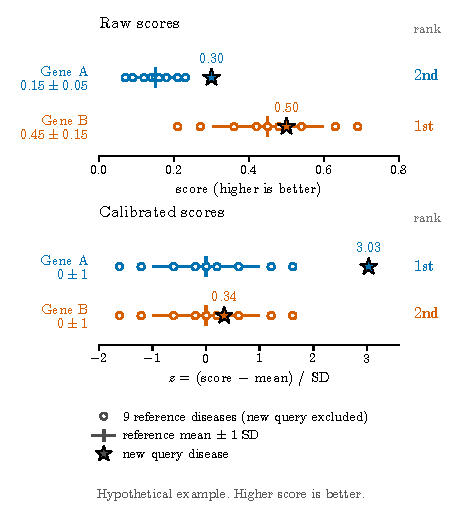
\includegraphics[width=\linewidth]{fig/fig_calibration.pdf}
\end{minipage}
\caption{Overview of \method{}.
(a) Solid arrows show training associations and annotations.
The dashed purple edge materializes the gene--disease--phenotype path
as a \texttt{causes\_phenotype} triple. The UPheno region groups
MP and HP phenotype classes; ontology hierarchy edges are omitted.
(b) Per-gene calibration. A candidate gene's score for the new disease is
standardized by subtracting that gene's mean and dividing by its standard
deviation over reference scores; the example illustrates the resulting rank
reversal. Evaluation uses one reference vector per distinct disease and
leaves out the query disease. A fixed training-disease panel is evaluated
separately.}
\label{fig:overview}
\end{figure*}


\section{Models and fixed configurations}

TransD \cite{ji2015knowledge} assigns each entity $e$ a pair of embeddings
$(e, \mathbf{w}_e) \in \mathbb{R}^d \times \mathbb{R}^d$ and each relation $r$
a pair $(r, \mathbf{w}_r) \in \mathbb{R}^k \times \mathbb{R}^k$. Its scoring
function is
\begin{equation}
  f(h, r, t) = -\bigl\|(\mathbf{w}_r \mathbf{w}_h^\top + \mathbf{I})\,h + r - (\mathbf{w}_r \mathbf{w}_t^\top + \mathbf{I})\,t\bigr\|_2^2,
  \label{eq:transd_supp}
\end{equation}
where $(\mathbf{w}_r \mathbf{w}_h^\top + \mathbf{I})$ and
$(\mathbf{w}_r \mathbf{w}_t^\top + \mathbf{I})$ are relation- and
entity-specific $k \times d$ projection matrices and $\mathbf{I}$ is the
$k \times d$ truncated identity. This projection supports the many-to-many
relations in the graph. TransD also performed well in related
gene-prioritization work \cite{indigena,althagafi2024prioritizing}.

ConvKB-D replaces TransD's translational scoring function with a convolutional
network applied to the stacked head, relation and tail embeddings, initialised
from pretrained TransD embeddings and then fine-tuned jointly with the filters.
We use it to test whether the conclusions depend on the scoring architecture.
The scoring function is:
\begin{equation}
  f(h, r, t) = \bigl[\,g(\omega_1 * [\mathbf{h}, \mathbf{r}, \mathbf{t}]);\,
    \dots;\, g(\omega_\tau * [\mathbf{h}, \mathbf{r}, \mathbf{t}])\,\bigr]
    \cdot \mathbf{w},
  \label{eq:convkb}
\end{equation}
where $[\mathbf{h}, \mathbf{r}, \mathbf{t}] \in \mathbb{R}^{d \times 3}$
stacks the three embeddings, each of the $\tau$ filters $\omega_j$ produces a
feature map through the non-linearity $g$, and $\mathbf{w}$ is a shared weight
vector projecting the concatenated feature maps to a scalar. The relation embedding enters as one column of the convolution input.


We run ConvKB-D on \method{}-pfs to compare the two embedding architectures
with all three annotation types. Both its calibrated and uncalibrated
procedures start from the same TransD checkpoint, selected using calibrated
validation mean rank for the matching fold and seed. Subsequent ConvKB-D
model selection, early stopping and test ranking use the respective calibrated
or uncalibrated scores. Initialising from a fold's own checkpoint matters: a model
started from fold 0 weights and evaluated on another fold would see, through its
initialisation, diseases that fold holds out.


Table~\ref{tab:configurations} gives the fixed configurations used in the
reruns. The TransD configurations are inherited from the historical manuscript/code
choices and frozen before these results. Their original selection used fold-0
validation diseases, the 4,399-gene pool, row calibration and history-dependent
projection. They were not retuned on the new pools or graphs. Excluding the
545 reconstructed fold-0 validation diseases (586 test associations) from
evaluation, while retaining the saved scores and reference panels, gives
LinkGDA mean-rank differences of -321.78, -48.74 and -543.31 from INDIGENA,
ConvKB-D and ULTRA, with the same adjusted significance decisions. Identity
with the historical validation split remains unverified. Each run retains
both raw- and calibrated-validation-selected checkpoints at that configuration.
The separate ConvKB-D configurations also remain fixed. Training uses Adam,
one uniformly sampled negative per positive, at most 1,000 epochs, validation
every 20 epochs, and patience of 15 validation evaluations. Typed negative
sampling is disabled. Main runs use seed 0; excluded runs use seeds 0--9.
All validation splits use seed 0. Excluded checkpoint selection retains only
validation pairs whose genes lack training associations and ranks them against
the full GO pool. The excluded seed-0 selection cohort has 333 validation pairs.

\begin{table}[htbp]
\centering\small
\caption{Fixed configurations. ConvKB-D has embedding dimension 200 and zero
hidden dropout; its calibrated and raw configurations use 100 and 200 filters,
respectively. The excluded f/fs variants use the corresponding TransD settings.}
\label{tab:configurations}
\begin{tabular}{lrrr}
\toprule
Method & Dimension & Batch size & Learning rate\\
\midrule
LinkGDA-p & 800 & 131072 & $10^{-4}$\\
LinkGDA-pf, -ps & 400 & 131072 & $10^{-3}$\\
LinkGDA-pfs, -f, -fs, -s & 200 & 65536 & $10^{-3}$\\
INDIGENA & 400 & 65536 & $10^{-3}$\\
ConvKB-D, calibrated & 200 & 65536 & $10^{-4}$\\
ConvKB-D, raw & 200 & 65536 & $10^{-3}$\\
\bottomrule
\end{tabular}
\end{table}

The semantic baselines compute Resnik-BMA, Lin-BMA and SimGIC on the shared
candidate and disease profiles. Exomiser v14.0.0 uses phenotype release 2406;
only its Phive phenotype score is a comparator. All 6,571 test associations
have 13,625 returned candidates, including the true gene. The true gene has
score zero for 694 associations (10.56\%). Per-query coverage is retained.
The older phenotype release gives Phive a different annotation coverage
from the study's prepared MGI profiles. ULTRA uses the released
\texttt{ultra\_4g.pth} checkpoint without fine-tuning. The pinned repository
revision and checkpoint digest are retained with its inference environment.

\begin{table*}[tb]
\centering\small
\caption{Raw and calibrated scores on the main pool, using the calibrated-selected checkpoint for trainable models. MR is fold mean $\pm$ sample standard deviation.}
\label{tab:raw_scores}
\begin{tabular}{lrrrr}
\toprule
Method & Scoring & MR & MRR & H@10 (\%) \\
\midrule
SimGIC & Raw & 3769.82\std{283.28} & 0.017 & 3.02 \\
SimGIC & Calibrated & 4004.83\std{271.76} & 0.020 & 3.99 \\
Resnik-BMA & Raw & 3222.61\std{255.65} & 0.031 & 6.82 \\
Resnik-BMA & Calibrated & 3129.78\std{211.95} & 0.022 & 4.48 \\
Lin-BMA & Raw & 3229.26\std{250.07} & 0.028 & 5.90 \\
Lin-BMA & Calibrated & 3132.24\std{214.93} & 0.017 & 3.65 \\
Exomiser-Phive & Raw & 3233.01\std{200.45} & 0.024 & 4.62 \\
Exomiser-Phive & Calibrated & 3730.72\std{190.94} & 0.005 & 0.73 \\
INDIGENA & Raw & 2133.22\std{199.89} & 0.039 & 9.14 \\
INDIGENA & Calibrated & 2048.30\std{159.92} & 0.033 & 6.97 \\
ULTRA, zero-shot & Raw & 2920.13\std{167.34} & 0.051 & 9.63 \\
ULTRA, zero-shot & Calibrated & 2274.28\std{113.84} & 0.045 & 9.13 \\
ConvKB-D & Raw & 2535.03\std{133.92} & 0.025 & 5.16 \\
ConvKB-D & Calibrated & 1779.94\std{148.43} & 0.033 & 7.17 \\
LinkGDA & Raw & 2538.18\std{115.76} & 0.023 & 4.96 \\
LinkGDA & Calibrated & 1729.37\std{142.91} & 0.026 & 5.61 \\
\bottomrule
\end{tabular}
\end{table*}


\section{Training-status controls}

The main annotation-defined pool has a random-order mean rank of 6,813.
Averaged over folds, ranking training-associated genes first gives 5,504.67;
ranking unseen genes first gives 8,121.33. Each group is tied internally.
These controls use the actual retained training associations after validation
withholding. Within-status evaluation reranks each query's true gene only
against candidates of the same status; it retains the original calibrated
scores. It is invariant to adding any constant score offset to either status
group, a property checked by a regression test with average-rank ties.

\begin{table*}[tb]
\centering\small
\caption{Mean rank after reranking only among candidates sharing the true gene's training-association status. Calibration retains the original reference panel. Fold-averaged random-order ranks are 1,890.1 for seen and 4,923.4 for unseen genes; there are 3,085 and 3,486 test pairs, respectively.}
\label{tab:status}
\begin{tabular}{lrr}
\toprule
Method & Seen genes & Unseen genes \\
\midrule
SimGIC & 1059.17 & 2896.61 \\
Resnik-BMA & 759.53 & 2502.67 \\
Lin-BMA & 753.87 & 2524.73 \\
Exomiser-Phive & 939.38 & 2915.83 \\
INDIGENA & 442.27 & 1769.88 \\
ULTRA, zero-shot & 434.71 & 1755.12 \\
ConvKB-D & 387.43 & 1574.17 \\
LinkGDA & 392.76 & 1427.17 \\
\bottomrule
\end{tabular}
\end{table*}


\begin{table*}[tb]
\centering\small
\caption{Exact mean-rank expectation when each association is scored against every other distinct disease in its fold or cohort. Calibration panels remain fixed. Averages give equal weight to folds or seeds. Random-order MR is 6,813 for main and 2,848.5 for no-MGI. This is a descriptive control.}
\label{tab:query_control}
\begin{tabular}{lrrrr}
\toprule
Model / pool & Raw: actual & Raw: other & Cal.: actual & Cal.: other \\
\midrule
Main: linkgda & 2538.18 & 4500.23 & 1729.37 & 6772.42 \\
Main: indigena & 2133.22 & 4981.38 & 2048.30 & 6800.56 \\
Main: convkb & 2535.03 & 4600.39 & 1779.94 & 6901.82 \\
Main: ultra & 2920.13 & 4513.28 & 2274.28 & 6966.29 \\
No-MGI: linkgda-f & 1083.36 & 2047.68 & 1192.91 & 2904.80 \\
No-MGI: linkgda-fs & 855.63 & 1629.65 & 1169.42 & 2846.13 \\
No-MGI: ultra-f & 1288.71 & 2275.27 & 1311.11 & 2979.06 \\
No-MGI: ultra-fs & 1203.60 & 2080.29 & 1471.22 & 3020.45 \\
\bottomrule
\end{tabular}
\end{table*}


Annotation-count controls rank all candidates by the number of distinct
prepared phenotype, function or expression annotations, in both directions,
without using the disease. Descriptive strata use a zero-annotation group
and positive-count quartiles defined across all candidate genes. Their ranks
remain ranks in the full candidate pool. Ranking larger phenotype, function
and expression annotation counts first gives main-pool mean ranks 4,211.92,
4,633.41 and 6,746.81, respectively. In the primary excluded pool, function
and expression counts give mean ranks 1,571.70 and 1,859.52, compared with
2,848.5 for tied scores. In the full-GO pool, placing genes without MGI
annotations first gives mean rank 2,848.5; the primary pool conditions on this
annotation status and ties every candidate under that rule. The count cutpoints, group sizes,
per-fold results and input hashes are retained in the annotation audit.

\section{Annotation-source sensitivity}

\begin{table*}[tb]
\centering\small
\caption{Annotation-source sensitivity on the 13,625-gene pool. Each variant uses its fixed configuration and calibrated-selected checkpoint; scoring uses disease-level leave-one-out calibration. SD is across ten folds.}
\label{tab:rq1_ablation}
\begin{tabular}{lrrr}
\toprule
Variant & MR & MRR & H@10 (\%) \\
\midrule
LinkGDA-p & 2699.33\std{99.03} & 0.025 & 5.11 \\
LinkGDA-f & 2409.68\std{137.96} & 0.029 & 5.69 \\
LinkGDA-s & 3748.19\std{122.67} & 0.020 & 3.69 \\
LinkGDA-pf & 1790.43\std{141.67} & 0.024 & 4.98 \\
LinkGDA-ps & 2181.59\std{138.84} & 0.023 & 4.70 \\
LinkGDA-fs & 2057.70\std{146.74} & 0.024 & 5.04 \\
LinkGDA-pfs & 1729.37\std{142.91} & 0.026 & 5.61 \\
\bottomrule
\end{tabular}
\end{table*}


The withheld-phenotype variants retain training associations and their
materialized gene--phenotype links. A gene without another represented
annotation retains its first eligible mouse phenotype edge. Among 13,625
main candidates, this fallback affects 418 genes for function alone,
1,175 for expression alone and 257 for function with expression. The
corresponding affected test-pair counts are 29, 426 and 15 of 6,571.
The excluded cohort's true genes lack MGI phenotypes and receive no fallback.

\section{Calibration and statistical comparisons}
\label{sec:calibration_comparisons}

\begin{table*}[tb]
\centering\small
\caption{Checkpoint selection and score calibration for LinkGDA-pfs at fixed hyperparameters. Values are equal-fold means. The fixed training reference contains one vector per distinct training disease.}
\label{tab:calibration}
\begin{tabular}{lrrr}
\toprule
Checkpoint & Scoring & MR & H@10 (\%) \\
\midrule
raw-selected & raw & 2540.61 & 5.11 \\
raw-selected & disease loo & 1721.23 & 5.68 \\
raw-selected & fixed training & 1717.77 & 5.84 \\
cal-selected & raw & 2538.18 & 4.96 \\
cal-selected & disease loo & 1729.37 & 5.61 \\
cal-selected & fixed training & 1721.63 & 5.82 \\
\bottomrule
\end{tabular}
\end{table*}


For each gene, leave-one-out calibration uses one vector per distinct other
test disease. The fixed-panel sensitivity uses one vector per training disease.
Both use population standard deviations and add $10^{-12}$ to the denominator.
Disease identities and candidate order accompany each fixed panel. Scores for
repeated occurrences of a disease must be identical. The full two-by-two
selection/scoring comparison and the fixed-panel result distinguish score
transformation from checkpoint choice. ConvKB-D's raw and calibrated arms
also differ in their frozen learning rate and filter count.

The original embedding-model comparison tests calibrated LinkGDA against INDIGENA,
ConvKB-D and zero-shot ULTRA on ten paired fold mean ranks. Two-sided Wilcoxon
$p$-values are 0.001953, 0.027344 and 0.001953; Holm-adjusted values are
0.005859, 0.027344 and 0.005859. Mean differences, LinkGDA minus comparator,
are $-318.93$, $-50.57$ and $-544.92$. The retained comparison JSON contains
all fold differences. These are fold-level comparisons conditional on the
shared training design; overlapping training sets limit independence, and
the benchmark also informed method development.

For excluded f and fs, we average each pair's ranks over ten seeds before
forming paired differences from deterministic ULTRA. Bootstrap samples draw
417 disease clusters with replacement and retain every association of each
sampled disease. We use 10,000 replicates, seed 20261013, and 97.5\% percentile
intervals for each of the two prespecified comparisons. The f difference is
$-118.20$ (interval $-252.84$ to $13.61$); the fs difference is $-301.80$
($-444.85$ to $-165.55$). Seed variation is reported separately as optimization
variability. Full-GO, alternative calibration, modalities, filtered ranking
and annotation strata are descriptive sensitivities.


\begin{table*}[tb]
\centering\small
\caption{Query-independent prepared-annotation count controls with average-rank ties. Primary and secondary denote the no-MGI and full-GO excluded pools.}
\label{tab:count_controls}
\begin{tabular}{lrrrrr}
\toprule
Pool & Count & Ordering & MR & H@10 (\%) & H@100 (\%) \\
\midrule
main & phenotype & More first & 4211.92 & 0.97 & 4.50 \\
main & phenotype & Fewer first & 9414.08 & 0.00 & 0.00 \\
main & function & More first & 4633.41 & 0.48 & 2.82 \\
main & function & Fewer first & 8992.59 & 0.00 & 0.00 \\
main & expression & More first & 6746.81 & 0.00 & 0.00 \\
main & expression & Fewer first & 6879.19 & 0.00 & 0.00 \\
primary & function & More first & 1571.70 & 0.24 & 6.35 \\
primary & function & Fewer first & 4125.30 & 0.00 & 0.00 \\
primary & expression & More first & 1859.52 & 0.00 & 0.00 \\
primary & expression & Fewer first & 3837.48 & 0.00 & 0.00 \\
secondary & function & More first & 8573.05 & 0.00 & 0.00 \\
secondary & function & Fewer first & 10331.95 & 0.00 & 0.00 \\
secondary & expression & More first & 7467.25 & 0.00 & 0.00 \\
secondary & expression & Fewer first & 11437.75 & 0.00 & 0.00 \\
\bottomrule
\end{tabular}
\end{table*}

\begin{table*}[tb]
\centering\small
\caption{Main-benchmark secondary metrics, averaged over folds. All scores use disease-level calibration. Hits are percentages; the final column averages within-fold or within-seed medians. The 1\% and 5\% thresholds are 137 and 682 candidates.}
\label{tab:secondary_main}
\resizebox{\textwidth}{!}{\begin{tabular}{lrrrrrrrr}
\toprule
Method & H@1 & H@3 & H@100 & H@1\% & H@5\% & Disease MR & Filtered MR & Median \\
\midrule
SimGIC & 0.76 & 1.82 & 14.28 & 16.53 & 33.85 & 3832.85 & 4004.53 & 2150.6 \\
Resnik-BMA & 0.75 & 1.86 & 18.58 & 22.21 & 42.07 & 3105.17 & 3129.48 & 1218.5 \\
Lin-BMA & 0.49 & 1.36 & 16.98 & 20.39 & 40.76 & 3120.99 & 3131.94 & 1223.0 \\
Phive & 0.15 & 0.26 & 6.48 & 8.81 & 29.45 & 3687.24 & 3730.42 & 2011.0 \\
INDIGENA & 1.08 & 2.87 & 28.78 & 32.95 & 55.15 & 2045.07 & 2048.00 & 475.1 \\
ULTRA & 1.82 & 3.92 & 34.35 & 39.07 & 58.71 & 2222.58 & 2273.98 & 326.9 \\
ConvKB-D & 1.10 & 2.50 & 30.03 & 34.76 & 57.97 & 1783.66 & 1779.64 & 399.4 \\
LinkGDA & 0.71 & 1.96 & 25.65 & 30.09 & 56.20 & 1709.56 & 1729.07 & 475.3 \\
\bottomrule
\end{tabular}}
\end{table*}

\begin{table*}[tb]
\centering\small
\caption{Primary excluded-cohort secondary metrics, averaged over seeds; ULTRA is deterministic. All scores use disease-level calibration. Hits are percentages; the final column averages within-fold or within-seed medians. The 1\% and 5\% thresholds are 57 and 285 candidates.}
\label{tab:secondary_primary}
\resizebox{\textwidth}{!}{\begin{tabular}{lrrrrrrrr}
\toprule
Method & H@1 & H@3 & H@100 & H@1\% & H@5\% & Disease MR & Filtered MR & Median \\
\midrule
LinkGDA-f & 3.13 & 6.68 & 31.06 & 24.96 & 45.25 & 1203.71 & 1192.89 & 408.4 \\
ULTRA-f & 1.88 & 6.12 & 31.53 & 26.35 & 43.06 & 1309.79 & 1311.09 & 578.0 \\
LinkGDA-fs & 2.19 & 4.33 & 24.54 & 18.56 & 39.81 & 1179.91 & 1169.40 & 520.4 \\
ULTRA-fs & 2.12 & 5.41 & 22.35 & 18.35 & 28.94 & 1467.18 & 1471.20 & 862.0 \\
\bottomrule
\end{tabular}}
\end{table*}


For the exact query control, we rank each true gene against every other distinct
disease vector in its fold or cohort and average these ranks. All associated
genes of a disease share the substituted query; linearity yields the expected
association-pair mean rank without Monte Carlo sampling. Calibration panels
remain fixed. This diagnostic uses no new training or significance test.
In the primary fs comparison, the incorrect-query difference is -174.32 ranks;
subtracting it from the observed -301.80 leaves -127.48 as the difference in
query-dependent rank improvement. For the main comparison with ConvKB-D,
incorrect-query ranks also favour LinkGDA, whereas the improvement from
incorrect to correct queries is slightly larger for ConvKB-D. These diagnostics
qualify what the prespecified predictive-rank comparisons establish.

The pooled main-benchmark median is 467 for LinkGDA, 312 for ULTRA, 394 for
ConvKB-D and 470 for INDIGENA. LinkGDA ranks higher on 46.16\%, 42.69\% and
49.46\% of pairs against those comparators, respectively. Cases ULTRA ranks
beyond 5,000 contribute -774.36 ranks to the pooled mean difference of -543.29;
the remaining cases contribute +231.08. The paired-rank diagnostic retains
all threshold calculations. Pooled pair weighting here differs from the
equal-fold weighting in the original embedding comparison.

Fixed training-disease calibration gives main MR 1,721.63 for LinkGDA,
2,040.37 for INDIGENA and 1,774.56 for ConvKB-D. In the primary excluded pool,
it gives 1,127.52 for LinkGDA-f and 1,014.46 for LinkGDA-fs. Fixed-panel scores
were not computed for ULTRA, the semantic methods or Phive, so this deployable
panel comparison covers only the trained embedding models. Candidate-specific
exclusion of a gene's own training diseases remains an unperformed sensitivity.

The historical excluded design appended 350 test genes to 4,399 established
genes. Putting those 350 first gives MR 175.5; putting the 674 genes without
training associations first gives 337.5. These historical diagnostics motivate
conditioning the current primary pool on missing MGI annotations.

\section{Controlled phenotype-query comparison}
\label{sec:controlled_query}

The controlled design crosses four graph/readout arms, two pretrained
initializations, seeds 0, 1 and 2, and ten outer folds. The four arms use pooling
with training disease bridges, pooling without disease nodes, conjunction
without disease nodes, and typed EQ conjunction without disease nodes.
All arms use the one-source QueryNBFNet phenotype projection, the same prepared
benchmark, and a fixed 500-update training budget. The ULTRA-initialized comparison
is prespecified as the main analysis. The UltraQuery-initialized comparison
measures the same component effects after logical-query pretraining.

For each training disease $d$, let $P'_d\subseteq P_d$ be the sampled set of at
most eight distinct phenotypes, and let $q(g,P'_d)$ be the pooling or conjunctive
readout for candidate gene $g$ over that set. Let $G^+(d)$ contain all known
positive candidate genes and $G^-(d)$ contain the sampled negatives. We optimize
\begin{equation}
\mathcal{L}(d)=
\log\!\left(\sum_{g\in G^+(d)\cup G^-(d)}\exp q(g,P'_d)\right)
-\frac{1}{|G^+(d)|}\sum_{g\in G^+(d)}q(g,P'_d).
\end{equation}
We sample 32 uniform negative candidates without replacement, then draw 256
proposals from the remaining negative candidates and retain the 32 with the
highest current scores. Ties are resolved by candidate identifier. Pooling uses
a sigmoid-transformed scalar weight initialized at 0.5; conjunction uses mean
log-sigmoid at unit temperature. Training uses AdamW with learning rate $10^{-5}$,
zero weight decay and gradient norm clipping at 1.0. Graph forwards run in
evaluation mode with parameter gradients enabled. The first pass computes
phenotype scores and the loss derivatives; the second pass accumulates the
corresponding parameter gradients one phenotype at a time.

Validation occurs at steps 0, 100, 200, 300, 400 and 500. A checkpoint must
preserve both initial validation Hits@1 and Hits@10 to become eligible; the
lexicographic selection order is Hits@10, Hits@1, MRR and negative mean rank.
Initialization remains available when no update improves the eligible selection.
The 240 selections are frozen together before outer-test inference. Both initial
and selected weights are retained, together with their validation matrices and
complete selection trajectories. The selected update is recorded for each fold,
arm and seed in the released selection metadata.
Tables~\ref{tab:controlled_query_full_ultra_4g}
and~\ref{tab:controlled_query_full_ultraquery} give all three seeds under both
scoring modes. Main Table~\ref{main-tab:controlled_query_contrasts} reports the
eight prespecified association-pooled calibrated Hits@10 contrasts, with
phenotype-profile-cluster intervals and the separate per-seed estimates.

The same fixed checkpoints enter the 42-condition bias analysis. Main
Table~\ref{main-tab:controlled_bias_summary} summarizes selected-checkpoint
Hits@10 across seeds for the full calibrated cohort, two scoring rules on the
zero-overlap cohort, and the combined protocol. Tables~\ref{tab:controlled_bias_ultra-4g-seed0}--\ref{tab:controlled_bias_ultraquery-seed2}
retain each seed and both checkpoint types, including mean rank and individual
changes to calibration references, causal-gene competition and profile weighting.
The accompanying machine-readable results retain all 48 variants and 42
conditions. These sensitivities describe the fitted models under the stated
scoring rules and populations; the eight prespecified contrasts remain the
primary inferential family.

\begin{landscape}
\begin{table*}[p]
\centering\footnotesize
\setlength{\tabcolsep}{3pt}
\caption{Complete ULTRA-initialized controlled-query results: native raw scores and per-gene calibrated scores, with both initial and validation-selected checkpoints. H@10 is given separately for all three seeds. Remaining columns give means $\pm$ sample standard deviations across seeds. All metrics pool the same 6,571 associations over ten folds.}
\label{tab:controlled_query_full_ultra_4g}
\begin{adjustbox}{max width=\linewidth}
\begin{tabular}{lllrrrrrrr}
\toprule
Graph/readout & Checkpoint & Scoring & H@10 Seed 0 & H@10 Seed 1 & H@10 Seed 2 & H@10 (\%) & H@1 (\%) & MRR & MR \\
\midrule
Disease bridges, Pool & initial & raw & 10.15 & 10.15 & 10.15 & $10.15\pm 0.00$ & $2.77\pm 0.00$ & $0.052\pm 0.000$ & $3052.5\pm 0.0$ \\
Disease bridges, Pool & initial & calibrated & 9.59 & 9.59 & 9.59 & $9.59\pm 0.00$ & $1.52\pm 0.00$ & $0.043\pm 0.000$ & $2154.2\pm 0.0$ \\
Disease bridges, Pool & selected & raw & 12.05 & 12.39 & 12.24 & $12.23\pm 0.17$ & $3.28\pm 0.10$ & $0.063\pm 0.002$ & $2436.9\pm 81.2$ \\
Disease bridges, Pool & selected & calibrated & 9.94 & 9.71 & 9.86 & $9.84\pm 0.12$ & $1.82\pm 0.03$ & $0.047\pm 0.000$ & $2241.8\pm 11.9$ \\
No disease bridges, Pool & initial & raw & 6.89 & 6.89 & 6.89 & $6.89\pm 0.00$ & $1.43\pm 0.00$ & $0.033\pm 0.000$ & $3309.4\pm 0.0$ \\
No disease bridges, Pool & initial & calibrated & 8.77 & 8.77 & 8.77 & $8.77\pm 0.00$ & $1.46\pm 0.00$ & $0.041\pm 0.000$ & $1969.2\pm 0.0$ \\
No disease bridges, Pool & selected & raw & 9.79 & 9.40 & 9.27 & $9.49\pm 0.27$ & $2.20\pm 0.08$ & $0.047\pm 0.001$ & $2961.8\pm 32.0$ \\
No disease bridges, Pool & selected & calibrated & 11.40 & 11.17 & 11.29 & $11.29\pm 0.11$ & $2.00\pm 0.02$ & $0.052\pm 0.000$ & $2138.3\pm 17.2$ \\
No disease bridges, AND & initial & raw & 4.79 & 4.79 & 4.79 & $4.79\pm 0.00$ & $1.10\pm 0.00$ & $0.024\pm 0.000$ & $3508.7\pm 0.0$ \\
No disease bridges, AND & initial & calibrated & 11.76 & 11.76 & 11.76 & $11.76\pm 0.00$ & $2.65\pm 0.00$ & $0.059\pm 0.000$ & $1869.5\pm 0.0$ \\
No disease bridges, AND & selected & raw & 4.93 & 5.10 & 4.79 & $4.94\pm 0.15$ & $1.12\pm 0.02$ & $0.025\pm 0.001$ & $3508.7\pm 3.3$ \\
No disease bridges, AND & selected & calibrated & 11.93 & 11.75 & 11.76 & $11.81\pm 0.10$ & $2.67\pm 0.02$ & $0.059\pm 0.000$ & $1875.7\pm 6.2$ \\
No disease bridges + typed EQ, AND & initial & raw & 7.75 & 7.75 & 7.75 & $7.75\pm 0.00$ & $2.22\pm 0.00$ & $0.041\pm 0.000$ & $3239.6\pm 0.0$ \\
No disease bridges + typed EQ, AND & initial & calibrated & 13.47 & 13.47 & 13.47 & $13.47\pm 0.00$ & $3.15\pm 0.00$ & $0.067\pm 0.000$ & $1766.0\pm 0.0$ \\
No disease bridges + typed EQ, AND & selected & raw & 8.32 & 8.14 & 7.91 & $8.13\pm 0.21$ & $2.28\pm 0.05$ & $0.043\pm 0.001$ & $3195.1\pm 19.2$ \\
No disease bridges + typed EQ, AND & selected & calibrated & 13.33 & 13.36 & 13.39 & $13.36\pm 0.03$ & $3.07\pm 0.02$ & $0.066\pm 0.000$ & $1792.5\pm 11.0$ \\
\bottomrule
\end{tabular}
\end{adjustbox}
\end{table*}
\clearpage
\begin{table*}[p]
\centering\footnotesize
\setlength{\tabcolsep}{3pt}
\caption{Complete UltraQuery-initialized controlled-query results: native raw scores and per-gene calibrated scores, with both initial and validation-selected checkpoints. H@10 is given separately for all three seeds. Remaining columns give means $\pm$ sample standard deviations across seeds. All metrics pool the same 6,571 associations over ten folds.}
\label{tab:controlled_query_full_ultraquery}
\begin{adjustbox}{max width=\linewidth}
\begin{tabular}{lllrrrrrrr}
\toprule
Graph/readout & Checkpoint & Scoring & H@10 Seed 0 & H@10 Seed 1 & H@10 Seed 2 & H@10 (\%) & H@1 (\%) & MRR & MR \\
\midrule
Disease bridges, Pool & initial & raw & 7.41 & 7.41 & 7.41 & $7.41\pm 0.00$ & $2.75\pm 0.00$ & $0.044\pm 0.000$ & $4340.6\pm 0.0$ \\
Disease bridges, Pool & initial & calibrated & 8.17 & 8.17 & 8.17 & $8.17\pm 0.00$ & $1.52\pm 0.00$ & $0.037\pm 0.000$ & $6220.4\pm 0.0$ \\
Disease bridges, Pool & selected & raw & 7.64 & 7.49 & 7.64 & $7.59\pm 0.09$ & $2.79\pm 0.04$ & $0.045\pm 0.000$ & $4172.6\pm 28.6$ \\
Disease bridges, Pool & selected & calibrated & 8.19 & 8.19 & 8.22 & $8.20\pm 0.02$ & $1.53\pm 0.01$ & $0.037\pm 0.000$ & $5891.3\pm 32.6$ \\
No disease bridges, Pool & initial & raw & 8.05 & 8.05 & 8.05 & $8.05\pm 0.00$ & $2.71\pm 0.00$ & $0.045\pm 0.000$ & $4461.9\pm 0.0$ \\
No disease bridges, Pool & initial & calibrated & 7.34 & 7.34 & 7.34 & $7.34\pm 0.00$ & $1.23\pm 0.00$ & $0.033\pm 0.000$ & $6306.4\pm 0.0$ \\
No disease bridges, Pool & selected & raw & 8.64 & 8.45 & 8.69 & $8.59\pm 0.13$ & $3.15\pm 0.02$ & $0.051\pm 0.001$ & $3773.3\pm 54.9$ \\
No disease bridges, Pool & selected & calibrated & 8.04 & 7.97 & 8.00 & $8.00\pm 0.03$ & $1.37\pm 0.05$ & $0.036\pm 0.001$ & $4271.2\pm 95.0$ \\
No disease bridges, AND & initial & raw & 9.04 & 9.04 & 9.04 & $9.04\pm 0.00$ & $3.50\pm 0.00$ & $0.054\pm 0.000$ & $4505.9\pm 0.0$ \\
No disease bridges, AND & initial & calibrated & 10.36 & 10.36 & 10.36 & $10.36\pm 0.00$ & $3.70\pm 0.00$ & $0.059\pm 0.000$ & $6379.6\pm 0.0$ \\
No disease bridges, AND & selected & raw & 9.02 & 9.12 & 8.99 & $9.04\pm 0.06$ & $3.42\pm 0.08$ & $0.054\pm 0.001$ & $3901.1\pm 73.9$ \\
No disease bridges, AND & selected & calibrated & 10.85 & 11.22 & 11.23 & $11.10\pm 0.22$ & $3.94\pm 0.08$ & $0.063\pm 0.001$ & $4492.1\pm 192.4$ \\
No disease bridges + typed EQ, AND & initial & raw & 11.57 & 11.57 & 11.57 & $11.57\pm 0.00$ & $4.02\pm 0.00$ & $0.066\pm 0.000$ & $3063.6\pm 0.0$ \\
No disease bridges + typed EQ, AND & initial & calibrated & 13.77 & 13.77 & 13.77 & $13.77\pm 0.00$ & $4.73\pm 0.00$ & $0.078\pm 0.000$ & $2438.6\pm 0.0$ \\
No disease bridges + typed EQ, AND & selected & raw & 11.67 & 11.58 & 11.95 & $11.73\pm 0.19$ & $4.09\pm 0.06$ & $0.066\pm 0.001$ & $3032.6\pm 16.9$ \\
No disease bridges + typed EQ, AND & selected & calibrated & 13.82 & 13.77 & 13.92 & $13.84\pm 0.08$ & $4.69\pm 0.08$ & $0.078\pm 0.000$ & $2334.4\pm 74.6$ \\
\bottomrule
\end{tabular}
\end{adjustbox}
\end{table*}
\clearpage
\end{landscape}

% Report SHA256: 5d38916427307922d9c837cedc4c0cd14d0e8fa9184730bbd9ed34b3c6ff526a
% Score manifest SHA256: a4940f8e8a0ed4d979276be92b518727aa75bd8d9242145277842350c8c68f8c
\begin{landscape}
\begin{table*}[p]
\centering\footnotesize
\setlength{\tabcolsep}{3pt}
\caption{ULTRA initialization, seed 0: bias sensitivities over ten folds and 13,625 candidates. Cells give H@10 (\%)/MR. Each seed is reported separately, with both initial and validation-selected checkpoints. Panel A: S0 uses raw scores; S1 applies per-gene calibration; S2 adds within-query training-status standardization. S0--S2 use 6,571 association pairs. Zero-overlap columns use 4,431 pairs; S4 combines reference deduplication, training-profile exclusion, co-causal filtering and equal-profile weighting (4,011 profiles). Panel B changes one operation relative to S1: reference deduplication and co-causal filtering retain 6,571 pairs, equal weighting uses their 5,928 profiles, and training-profile exclusion retains 6,361 pairs. These scoring, competition, weighting and population changes are descriptive sensitivities under the specified protocols. The accompanying CSV retains every variant, all 42 conditions, exact metric values and population units.}
\label{tab:controlled_bias_ultra-4g-seed0}
\textbf{Panel A: scoring adjustments and evaluation cohorts}\par\smallskip
\begin{adjustbox}{max width=\linewidth}
\begin{tabular}{lrrrrrr}
\toprule
Configuration & S0: raw & S1: calibrated & S2: status-Z & Zero overlap: raw & S3: status-Z & S4: combined \\
\midrule
Disease bridges, Pool, initial & 10.15 / 3052.5 & 9.59 / 2154.2 & 9.40 / 1999.5 & 0.14 / 4415.5 & 8.69 / 2650.3 & 9.37 / 2621.2 \\
Disease bridges, Pool, selected & 12.05 / 2526.2 & 9.94 / 2233.4 & 9.71 / 2027.6 & 0.43 / 3656.6 & 9.30 / 2699.5 & 9.93 / 2706.0 \\
No disease bridges, Pool, initial & 6.89 / 3309.4 & 8.77 / 1969.2 & 8.70 / 1951.9 & 0.32 / 4730.3 & 7.09 / 2568.7 & 7.50 / 2519.2 \\
No disease bridges, Pool, selected & 9.79 / 2924.9 & 11.40 / 2150.6 & 10.12 / 1954.3 & 0.50 / 4225.1 & 12.21 / 2597.3 & 12.86 / 2591.1 \\
No disease bridges, AND, initial & 4.79 / 3508.7 & 11.76 / 1869.5 & 11.31 / 1845.7 & 0.29 / 4892.5 & 13.34 / 2384.2 & 14.11 / 2326.3 \\
No disease bridges, AND, selected & 4.93 / 3505.4 & 11.93 / 1875.7 & 11.22 / 1849.0 & 0.29 / 4891.8 & 13.32 / 2390.1 & 14.20 / 2334.4 \\
No disease bridges + typed EQ, AND, initial & 7.75 / 3239.6 & 13.47 / 1766.0 & 12.42 / 1699.7 & 0.36 / 4615.3 & 14.01 / 2204.2 & 14.83 / 2136.0 \\
No disease bridges + typed EQ, AND, selected & 8.32 / 3177.6 & 13.33 / 1805.1 & 12.33 / 1707.5 & 0.32 / 4535.5 & 13.77 / 2214.6 & 14.29 / 2148.6 \\
\bottomrule
\end{tabular}
\end{adjustbox}
\par\medskip
\textbf{Panel B: individual changes relative to S1}\par\smallskip
\begin{adjustbox}{max width=\linewidth}
\begin{tabular}{lrrrrr}
\toprule
Configuration & S1 reference & \shortstack{Deduplicate\\reference profiles} & \shortstack{Filter other\\causal genes} & \shortstack{Equal profile\\weights} & \shortstack{Exclude training-\\profile matches} \\
\midrule
Disease bridges, Pool, initial & 9.59 / 2154.2 & 9.56 / 2153.9 & 9.63 / 2153.9 & 9.85 / 2107.2 & 9.67 / 2166.1 \\
Disease bridges, Pool, selected & 9.94 / 2233.4 & 9.85 / 2234.4 & 9.95 / 2233.1 & 10.16 / 2205.4 & 10.01 / 2248.9 \\
No disease bridges, Pool, initial & 8.77 / 1969.2 & 8.70 / 1967.6 & 8.81 / 1968.9 & 8.98 / 1939.4 & 8.85 / 1979.1 \\
No disease bridges, Pool, selected & 11.40 / 2150.6 & 11.43 / 2153.3 & 11.40 / 2150.3 & 11.57 / 2119.6 & 11.41 / 2166.1 \\
No disease bridges, AND, initial & 11.76 / 1869.5 & 11.63 / 1864.9 & 11.76 / 1869.2 & 12.35 / 1831.5 & 11.98 / 1876.7 \\
No disease bridges, AND, selected & 11.93 / 1875.7 & 11.79 / 1871.1 & 11.96 / 1875.3 & 12.52 / 1839.3 & 12.12 / 1884.4 \\
No disease bridges + typed EQ, AND, initial & 13.47 / 1766.0 & 13.62 / 1760.3 & 13.51 / 1765.7 & 13.98 / 1713.0 & 13.74 / 1768.4 \\
No disease bridges + typed EQ, AND, selected & 13.33 / 1805.1 & 13.39 / 1799.0 & 13.36 / 1804.8 & 13.86 / 1746.1 & 13.60 / 1806.8 \\
\bottomrule
\end{tabular}
\end{adjustbox}
\end{table*}
\clearpage
\end{landscape}

% Report SHA256: 5d38916427307922d9c837cedc4c0cd14d0e8fa9184730bbd9ed34b3c6ff526a
% Score manifest SHA256: a4940f8e8a0ed4d979276be92b518727aa75bd8d9242145277842350c8c68f8c
\begin{landscape}
\begin{table*}[p]
\centering\footnotesize
\setlength{\tabcolsep}{3pt}
\caption{ULTRA initialization, seed 1: bias sensitivities over ten folds and 13,625 candidates. Cells give H@10 (\%)/MR. Each seed is reported separately, with both initial and validation-selected checkpoints. Panel A: S0 uses raw scores; S1 applies per-gene calibration; S2 adds within-query training-status standardization. S0--S2 use 6,571 association pairs. Zero-overlap columns use 4,431 pairs; S4 combines reference deduplication, training-profile exclusion, co-causal filtering and equal-profile weighting (4,011 profiles). Panel B changes one operation relative to S1: reference deduplication and co-causal filtering retain 6,571 pairs, equal weighting uses their 5,928 profiles, and training-profile exclusion retains 6,361 pairs. These scoring, competition, weighting and population changes are descriptive sensitivities under the specified protocols. The accompanying CSV retains every variant, all 42 conditions, exact metric values and population units.}
\label{tab:controlled_bias_ultra-4g-seed1}
\textbf{Panel A: scoring adjustments and evaluation cohorts}\par\smallskip
\begin{adjustbox}{max width=\linewidth}
\begin{tabular}{lrrrrrr}
\toprule
Configuration & S0: raw & S1: calibrated & S2: status-Z & Zero overlap: raw & S3: status-Z & S4: combined \\
\midrule
Disease bridges, Pool, initial & 10.15 / 3052.5 & 9.59 / 2154.2 & 9.40 / 1999.5 & 0.14 / 4415.5 & 8.69 / 2650.3 & 9.37 / 2621.2 \\
Disease bridges, Pool, selected & 12.39 / 2367.5 & 9.71 / 2255.4 & 9.48 / 2028.2 & 0.41 / 3424.9 & 9.37 / 2701.5 & 9.99 / 2712.4 \\
No disease bridges, Pool, initial & 6.89 / 3309.4 & 8.77 / 1969.2 & 8.70 / 1951.9 & 0.32 / 4730.3 & 7.09 / 2568.7 & 7.50 / 2519.2 \\
No disease bridges, Pool, selected & 9.40 / 2981.9 & 11.17 / 2145.7 & 10.11 / 1962.1 & 0.36 / 4300.8 & 11.65 / 2609.5 & 12.36 / 2599.5 \\
No disease bridges, AND, initial & 4.79 / 3508.7 & 11.76 / 1869.5 & 11.31 / 1845.7 & 0.29 / 4892.5 & 13.34 / 2384.2 & 14.11 / 2326.3 \\
No disease bridges, AND, selected & 5.10 / 3512.1 & 11.75 / 1882.0 & 11.19 / 1847.0 & 0.36 / 4906.6 & 13.32 / 2384.2 & 14.06 / 2334.6 \\
No disease bridges + typed EQ, AND, initial & 7.75 / 3239.6 & 13.47 / 1766.0 & 12.42 / 1699.7 & 0.36 / 4615.3 & 14.01 / 2204.2 & 14.83 / 2136.0 \\
No disease bridges + typed EQ, AND, selected & 8.14 / 3192.0 & 13.36 / 1784.7 & 12.27 / 1697.5 & 0.36 / 4552.2 & 13.83 / 2200.6 & 14.66 / 2137.6 \\
\bottomrule
\end{tabular}
\end{adjustbox}
\par\medskip
\textbf{Panel B: individual changes relative to S1}\par\smallskip
\begin{adjustbox}{max width=\linewidth}
\begin{tabular}{lrrrrr}
\toprule
Configuration & S1 reference & \shortstack{Deduplicate\\reference profiles} & \shortstack{Filter other\\causal genes} & \shortstack{Equal profile\\weights} & \shortstack{Exclude training-\\profile matches} \\
\midrule
Disease bridges, Pool, initial & 9.59 / 2154.2 & 9.56 / 2153.9 & 9.63 / 2153.9 & 9.85 / 2107.2 & 9.67 / 2166.1 \\
Disease bridges, Pool, selected & 9.71 / 2255.4 & 9.66 / 2257.5 & 9.72 / 2255.1 & 9.87 / 2225.8 & 9.76 / 2270.8 \\
No disease bridges, Pool, initial & 8.77 / 1969.2 & 8.70 / 1967.6 & 8.81 / 1968.9 & 8.98 / 1939.4 & 8.85 / 1979.1 \\
No disease bridges, Pool, selected & 11.17 / 2145.7 & 11.14 / 2148.3 & 11.22 / 2145.4 & 11.34 / 2110.5 & 11.18 / 2159.6 \\
No disease bridges, AND, initial & 11.76 / 1869.5 & 11.63 / 1864.9 & 11.76 / 1869.2 & 12.35 / 1831.5 & 11.98 / 1876.7 \\
No disease bridges, AND, selected & 11.75 / 1882.0 & 11.63 / 1877.2 & 11.76 / 1881.7 & 12.26 / 1843.4 & 11.93 / 1888.7 \\
No disease bridges + typed EQ, AND, initial & 13.47 / 1766.0 & 13.62 / 1760.3 & 13.51 / 1765.7 & 13.98 / 1713.0 & 13.74 / 1768.4 \\
No disease bridges + typed EQ, AND, selected & 13.36 / 1784.7 & 13.38 / 1779.0 & 13.41 / 1784.3 & 13.88 / 1725.9 & 13.63 / 1786.1 \\
\bottomrule
\end{tabular}
\end{adjustbox}
\end{table*}
\clearpage
\end{landscape}

% Report SHA256: 5d38916427307922d9c837cedc4c0cd14d0e8fa9184730bbd9ed34b3c6ff526a
% Score manifest SHA256: a4940f8e8a0ed4d979276be92b518727aa75bd8d9242145277842350c8c68f8c
\begin{landscape}
\begin{table*}[p]
\centering\footnotesize
\setlength{\tabcolsep}{3pt}
\caption{ULTRA initialization, seed 2: bias sensitivities over ten folds and 13,625 candidates. Cells give H@10 (\%)/MR. Each seed is reported separately, with both initial and validation-selected checkpoints. Panel A: S0 uses raw scores; S1 applies per-gene calibration; S2 adds within-query training-status standardization. S0--S2 use 6,571 association pairs. Zero-overlap columns use 4,431 pairs; S4 combines reference deduplication, training-profile exclusion, co-causal filtering and equal-profile weighting (4,011 profiles). Panel B changes one operation relative to S1: reference deduplication and co-causal filtering retain 6,571 pairs, equal weighting uses their 5,928 profiles, and training-profile exclusion retains 6,361 pairs. These scoring, competition, weighting and population changes are descriptive sensitivities under the specified protocols. The accompanying CSV retains every variant, all 42 conditions, exact metric values and population units.}
\label{tab:controlled_bias_ultra-4g-seed2}
\textbf{Panel A: scoring adjustments and evaluation cohorts}\par\smallskip
\begin{adjustbox}{max width=\linewidth}
\begin{tabular}{lrrrrrr}
\toprule
Configuration & S0: raw & S1: calibrated & S2: status-Z & Zero overlap: raw & S3: status-Z & S4: combined \\
\midrule
Disease bridges, Pool, initial & 10.15 / 3052.5 & 9.59 / 2154.2 & 9.40 / 1999.5 & 0.14 / 4415.5 & 8.69 / 2650.3 & 9.37 / 2621.2 \\
Disease bridges, Pool, selected & 12.24 / 2417.0 & 9.86 / 2236.6 & 9.72 / 2023.2 & 0.36 / 3498.0 & 9.46 / 2693.6 & 9.91 / 2703.1 \\
No disease bridges, Pool, initial & 6.89 / 3309.4 & 8.77 / 1969.2 & 8.70 / 1951.9 & 0.32 / 4730.3 & 7.09 / 2568.7 & 7.50 / 2519.2 \\
No disease bridges, Pool, selected & 9.27 / 2978.5 & 11.29 / 2118.6 & 10.23 / 1938.9 & 0.41 / 4296.1 & 11.96 / 2571.7 & 12.47 / 2560.6 \\
No disease bridges, AND, initial & 4.79 / 3508.7 & 11.76 / 1869.5 & 11.31 / 1845.7 & 0.29 / 4892.5 & 13.34 / 2384.2 & 14.11 / 2326.3 \\
No disease bridges, AND, selected & 4.79 / 3508.7 & 11.76 / 1869.5 & 11.31 / 1845.7 & 0.29 / 4892.5 & 13.34 / 2384.2 & 14.11 / 2326.3 \\
No disease bridges + typed EQ, AND, initial & 7.75 / 3239.6 & 13.47 / 1766.0 & 12.42 / 1699.7 & 0.36 / 4615.3 & 14.01 / 2204.2 & 14.83 / 2136.0 \\
No disease bridges + typed EQ, AND, selected & 7.91 / 3215.6 & 13.39 / 1787.8 & 12.34 / 1704.8 & 0.36 / 4585.0 & 13.81 / 2211.2 & 14.54 / 2145.1 \\
\bottomrule
\end{tabular}
\end{adjustbox}
\par\medskip
\textbf{Panel B: individual changes relative to S1}\par\smallskip
\begin{adjustbox}{max width=\linewidth}
\begin{tabular}{lrrrrr}
\toprule
Configuration & S1 reference & \shortstack{Deduplicate\\reference profiles} & \shortstack{Filter other\\causal genes} & \shortstack{Equal profile\\weights} & \shortstack{Exclude training-\\profile matches} \\
\midrule
Disease bridges, Pool, initial & 9.59 / 2154.2 & 9.56 / 2153.9 & 9.63 / 2153.9 & 9.85 / 2107.2 & 9.67 / 2166.1 \\
Disease bridges, Pool, selected & 9.86 / 2236.6 & 9.82 / 2238.1 & 9.88 / 2236.3 & 10.05 / 2208.8 & 9.90 / 2253.0 \\
No disease bridges, Pool, initial & 8.77 / 1969.2 & 8.70 / 1967.6 & 8.81 / 1968.9 & 8.98 / 1939.4 & 8.85 / 1979.1 \\
No disease bridges, Pool, selected & 11.29 / 2118.6 & 11.16 / 2121.4 & 11.29 / 2118.3 & 11.39 / 2086.9 & 11.29 / 2128.8 \\
No disease bridges, AND, initial & 11.76 / 1869.5 & 11.63 / 1864.9 & 11.76 / 1869.2 & 12.35 / 1831.5 & 11.98 / 1876.7 \\
No disease bridges, AND, selected & 11.76 / 1869.5 & 11.63 / 1864.9 & 11.76 / 1869.2 & 12.35 / 1831.5 & 11.98 / 1876.7 \\
No disease bridges + typed EQ, AND, initial & 13.47 / 1766.0 & 13.62 / 1760.3 & 13.51 / 1765.7 & 13.98 / 1713.0 & 13.74 / 1768.4 \\
No disease bridges + typed EQ, AND, selected & 13.39 / 1787.8 & 13.50 / 1781.9 & 13.44 / 1787.5 & 13.90 / 1728.0 & 13.66 / 1789.3 \\
\bottomrule
\end{tabular}
\end{adjustbox}
\end{table*}
\clearpage
\end{landscape}

% Report SHA256: 5d38916427307922d9c837cedc4c0cd14d0e8fa9184730bbd9ed34b3c6ff526a
% Score manifest SHA256: a4940f8e8a0ed4d979276be92b518727aa75bd8d9242145277842350c8c68f8c
\begin{landscape}
\begin{table*}[p]
\centering\footnotesize
\setlength{\tabcolsep}{3pt}
\caption{UltraQuery initialization, seed 0: bias sensitivities over ten folds and 13,625 candidates. Cells give H@10 (\%)/MR. Each seed is reported separately, with both initial and validation-selected checkpoints. Panel A: S0 uses raw scores; S1 applies per-gene calibration; S2 adds within-query training-status standardization. S0--S2 use 6,571 association pairs. Zero-overlap columns use 4,431 pairs; S4 combines reference deduplication, training-profile exclusion, co-causal filtering and equal-profile weighting (4,011 profiles). Panel B changes one operation relative to S1: reference deduplication and co-causal filtering retain 6,571 pairs, equal weighting uses their 5,928 profiles, and training-profile exclusion retains 6,361 pairs. These scoring, competition, weighting and population changes are descriptive sensitivities under the specified protocols. The accompanying CSV retains every variant, all 42 conditions, exact metric values and population units.}
\label{tab:controlled_bias_ultraquery-seed0}
\textbf{Panel A: scoring adjustments and evaluation cohorts}\par\smallskip
\begin{adjustbox}{max width=\linewidth}
\begin{tabular}{lrrrrrr}
\toprule
Configuration & S0: raw & S1: calibrated & S2: status-Z & Zero overlap: raw & S3: status-Z & S4: combined \\
\midrule
Disease bridges, Pool, initial & 7.41 / 4340.6 & 8.17 / 6220.4 & 7.93 / 6267.9 & 0.00 / 6317.8 & 0.09 / 8989.1 & 0.07 / 9021.0 \\
Disease bridges, Pool, selected & 7.64 / 4152.8 & 8.19 / 5869.3 & 7.84 / 5905.8 & 0.00 / 6042.4 & 0.20 / 8453.4 & 0.19 / 8516.1 \\
No disease bridges, Pool, initial & 8.05 / 4461.9 & 7.34 / 6306.4 & 7.23 / 6389.3 & 0.00 / 6474.0 & 0.18 / 9139.7 & 0.14 / 9189.3 \\
No disease bridges, Pool, selected & 8.64 / 3710.1 & 8.04 / 4162.5 & 6.91 / 4145.6 & 0.11 / 5381.5 & 0.93 / 5838.1 & 0.98 / 5811.7 \\
No disease bridges, AND, initial & 9.04 / 4505.9 & 10.36 / 6379.6 & 10.11 / 6340.1 & 0.02 / 5909.6 & 0.16 / 8855.9 & 0.15 / 8889.4 \\
No disease bridges, AND, selected & 9.02 / 3986.4 & 10.85 / 4714.3 & 10.79 / 4678.8 & 0.05 / 5508.0 & 0.93 / 6439.5 & 0.96 / 6372.6 \\
No disease bridges + typed EQ, AND, initial & 11.57 / 3063.6 & 13.77 / 2438.6 & 12.68 / 2438.9 & 0.11 / 4406.2 & 2.93 / 3302.8 & 3.04 / 3222.8 \\
No disease bridges + typed EQ, AND, selected & 11.67 / 3036.4 & 13.82 / 2348.6 & 12.65 / 2350.5 & 0.14 / 4368.1 & 3.18 / 3173.2 & 3.30 / 3104.4 \\
\bottomrule
\end{tabular}
\end{adjustbox}
\par\medskip
\textbf{Panel B: individual changes relative to S1}\par\smallskip
\begin{adjustbox}{max width=\linewidth}
\begin{tabular}{lrrrrr}
\toprule
Configuration & S1 reference & \shortstack{Deduplicate\\reference profiles} & \shortstack{Filter other\\causal genes} & \shortstack{Equal profile\\weights} & \shortstack{Exclude training-\\profile matches} \\
\midrule
Disease bridges, Pool, initial & 8.17 / 6220.4 & 8.22 / 6220.5 & 8.22 / 6220.1 & 8.00 / 6215.4 & 8.21 / 6203.1 \\
Disease bridges, Pool, selected & 8.19 / 5869.3 & 8.23 / 5869.3 & 8.23 / 5869.0 & 8.02 / 5894.7 & 8.22 / 5850.2 \\
No disease bridges, Pool, initial & 7.34 / 6306.4 & 7.44 / 6305.4 & 7.41 / 6306.1 & 7.11 / 6305.5 & 7.36 / 6289.1 \\
No disease bridges, Pool, selected & 8.04 / 4162.5 & 8.02 / 4164.3 & 8.10 / 4162.2 & 7.81 / 4160.2 & 8.05 / 4183.2 \\
No disease bridges, AND, initial & 10.36 / 6379.6 & 10.41 / 6372.8 & 10.44 / 6379.3 & 10.23 / 6364.5 & 10.53 / 6378.2 \\
No disease bridges, AND, selected & 10.85 / 4714.3 & 10.93 / 4713.7 & 10.91 / 4713.9 & 10.73 / 4655.1 & 11.04 / 4718.2 \\
No disease bridges + typed EQ, AND, initial & 13.77 / 2438.6 & 13.74 / 2434.2 & 13.80 / 2438.3 & 13.59 / 2419.4 & 13.99 / 2442.1 \\
No disease bridges + typed EQ, AND, selected & 13.82 / 2348.6 & 13.79 / 2344.7 & 13.85 / 2348.2 & 13.63 / 2335.5 & 14.04 / 2352.4 \\
\bottomrule
\end{tabular}
\end{adjustbox}
\end{table*}
\clearpage
\end{landscape}

% Report SHA256: 5d38916427307922d9c837cedc4c0cd14d0e8fa9184730bbd9ed34b3c6ff526a
% Score manifest SHA256: a4940f8e8a0ed4d979276be92b518727aa75bd8d9242145277842350c8c68f8c
\begin{landscape}
\begin{table*}[p]
\centering\footnotesize
\setlength{\tabcolsep}{3pt}
\caption{UltraQuery initialization, seed 1: bias sensitivities over ten folds and 13,625 candidates. Cells give H@10 (\%)/MR. Each seed is reported separately, with both initial and validation-selected checkpoints. Panel A: S0 uses raw scores; S1 applies per-gene calibration; S2 adds within-query training-status standardization. S0--S2 use 6,571 association pairs. Zero-overlap columns use 4,431 pairs; S4 combines reference deduplication, training-profile exclusion, co-causal filtering and equal-profile weighting (4,011 profiles). Panel B changes one operation relative to S1: reference deduplication and co-causal filtering retain 6,571 pairs, equal weighting uses their 5,928 profiles, and training-profile exclusion retains 6,361 pairs. These scoring, competition, weighting and population changes are descriptive sensitivities under the specified protocols. The accompanying CSV retains every variant, all 42 conditions, exact metric values and population units.}
\label{tab:controlled_bias_ultraquery-seed1}
\textbf{Panel A: scoring adjustments and evaluation cohorts}\par\smallskip
\begin{adjustbox}{max width=\linewidth}
\begin{tabular}{lrrrrrr}
\toprule
Configuration & S0: raw & S1: calibrated & S2: status-Z & Zero overlap: raw & S3: status-Z & S4: combined \\
\midrule
Disease bridges, Pool, initial & 7.41 / 4340.6 & 8.17 / 6220.4 & 7.93 / 6267.9 & 0.00 / 6317.8 & 0.09 / 8989.1 & 0.07 / 9021.0 \\
Disease bridges, Pool, selected & 7.49 / 4205.4 & 8.19 / 5928.8 & 8.02 / 5971.4 & 0.00 / 6119.6 & 0.20 / 8550.2 & 0.19 / 8601.6 \\
No disease bridges, Pool, initial & 8.05 / 4461.9 & 7.34 / 6306.4 & 7.23 / 6389.3 & 0.00 / 6474.0 & 0.18 / 9139.7 & 0.14 / 9189.3 \\
No disease bridges, Pool, selected & 8.45 / 3801.4 & 7.97 / 4311.9 & 7.35 / 4336.1 & 0.14 / 5516.5 & 0.47 / 6108.6 & 0.43 / 6118.9 \\
No disease bridges, AND, initial & 9.04 / 4505.9 & 10.36 / 6379.6 & 10.11 / 6340.1 & 0.02 / 5909.6 & 0.16 / 8855.9 & 0.15 / 8889.4 \\
No disease bridges, AND, selected & 9.12 / 3859.7 & 11.22 / 4377.2 & 11.08 / 4308.9 & 0.05 / 5377.7 & 1.06 / 5912.3 & 1.17 / 5860.7 \\
No disease bridges + typed EQ, AND, initial & 11.57 / 3063.6 & 13.77 / 2438.6 & 12.68 / 2438.9 & 0.11 / 4406.2 & 2.93 / 3302.8 & 3.04 / 3222.8 \\
No disease bridges + typed EQ, AND, selected & 11.58 / 3047.4 & 13.77 / 2400.8 & 12.71 / 2403.4 & 0.11 / 4383.1 & 3.07 / 3250.6 & 3.23 / 3173.3 \\
\bottomrule
\end{tabular}
\end{adjustbox}
\par\medskip
\textbf{Panel B: individual changes relative to S1}\par\smallskip
\begin{adjustbox}{max width=\linewidth}
\begin{tabular}{lrrrrr}
\toprule
Configuration & S1 reference & \shortstack{Deduplicate\\reference profiles} & \shortstack{Filter other\\causal genes} & \shortstack{Equal profile\\weights} & \shortstack{Exclude training-\\profile matches} \\
\midrule
Disease bridges, Pool, initial & 8.17 / 6220.4 & 8.22 / 6220.5 & 8.22 / 6220.1 & 8.00 / 6215.4 & 8.21 / 6203.1 \\
Disease bridges, Pool, selected & 8.19 / 5928.8 & 8.23 / 5928.9 & 8.23 / 5928.5 & 8.01 / 5947.6 & 8.22 / 5909.9 \\
No disease bridges, Pool, initial & 7.34 / 6306.4 & 7.44 / 6305.4 & 7.41 / 6306.1 & 7.11 / 6305.5 & 7.36 / 6289.1 \\
No disease bridges, Pool, selected & 7.97 / 4311.9 & 8.02 / 4313.2 & 8.04 / 4311.6 & 7.76 / 4336.5 & 8.02 / 4326.8 \\
No disease bridges, AND, initial & 10.36 / 6379.6 & 10.41 / 6372.8 & 10.44 / 6379.3 & 10.23 / 6364.5 & 10.53 / 6378.2 \\
No disease bridges, AND, selected & 11.22 / 4377.2 & 11.32 / 4378.5 & 11.28 / 4376.9 & 11.14 / 4328.9 & 11.43 / 4373.1 \\
No disease bridges + typed EQ, AND, initial & 13.77 / 2438.6 & 13.74 / 2434.2 & 13.80 / 2438.3 & 13.59 / 2419.4 & 13.99 / 2442.1 \\
No disease bridges + typed EQ, AND, selected & 13.77 / 2400.8 & 13.74 / 2396.7 & 13.82 / 2400.5 & 13.59 / 2386.5 & 13.99 / 2403.4 \\
\bottomrule
\end{tabular}
\end{adjustbox}
\end{table*}
\clearpage
\end{landscape}

% Report SHA256: 5d38916427307922d9c837cedc4c0cd14d0e8fa9184730bbd9ed34b3c6ff526a
% Score manifest SHA256: a4940f8e8a0ed4d979276be92b518727aa75bd8d9242145277842350c8c68f8c
\begin{landscape}
\begin{table*}[p]
\centering\footnotesize
\setlength{\tabcolsep}{3pt}
\caption{UltraQuery initialization, seed 2: bias sensitivities over ten folds and 13,625 candidates. Cells give H@10 (\%)/MR. Each seed is reported separately, with both initial and validation-selected checkpoints. Panel A: S0 uses raw scores; S1 applies per-gene calibration; S2 adds within-query training-status standardization. S0--S2 use 6,571 association pairs. Zero-overlap columns use 4,431 pairs; S4 combines reference deduplication, training-profile exclusion, co-causal filtering and equal-profile weighting (4,011 profiles). Panel B changes one operation relative to S1: reference deduplication and co-causal filtering retain 6,571 pairs, equal weighting uses their 5,928 profiles, and training-profile exclusion retains 6,361 pairs. These scoring, competition, weighting and population changes are descriptive sensitivities under the specified protocols. The accompanying CSV retains every variant, all 42 conditions, exact metric values and population units.}
\label{tab:controlled_bias_ultraquery-seed2}
\textbf{Panel A: scoring adjustments and evaluation cohorts}\par\smallskip
\begin{adjustbox}{max width=\linewidth}
\begin{tabular}{lrrrrrr}
\toprule
Configuration & S0: raw & S1: calibrated & S2: status-Z & Zero overlap: raw & S3: status-Z & S4: combined \\
\midrule
Disease bridges, Pool, initial & 7.41 / 4340.6 & 8.17 / 6220.4 & 7.93 / 6267.9 & 0.00 / 6317.8 & 0.09 / 8989.1 & 0.07 / 9021.0 \\
Disease bridges, Pool, selected & 7.64 / 4159.6 & 8.22 / 5875.7 & 7.88 / 5916.2 & 0.02 / 6052.5 & 0.23 / 8468.8 & 0.22 / 8528.3 \\
No disease bridges, Pool, initial & 8.05 / 4461.9 & 7.34 / 6306.4 & 7.23 / 6389.3 & 0.00 / 6474.0 & 0.18 / 9139.7 & 0.14 / 9189.3 \\
No disease bridges, Pool, selected & 8.69 / 3808.4 & 8.00 / 4339.0 & 7.46 / 4342.3 & 0.07 / 5525.7 & 0.79 / 6109.9 & 0.76 / 6082.6 \\
No disease bridges, AND, initial & 9.04 / 4505.9 & 10.36 / 6379.6 & 10.11 / 6340.1 & 0.02 / 5909.6 & 0.16 / 8855.9 & 0.15 / 8889.4 \\
No disease bridges, AND, selected & 8.99 / 3857.1 & 11.23 / 4384.9 & 11.03 / 4336.7 & 0.02 / 5388.7 & 0.99 / 5961.9 & 1.06 / 5871.6 \\
No disease bridges + typed EQ, AND, initial & 11.57 / 3063.6 & 13.77 / 2438.6 & 12.68 / 2438.9 & 0.11 / 4406.2 & 2.93 / 3302.8 & 3.04 / 3222.8 \\
No disease bridges + typed EQ, AND, selected & 11.95 / 3014.1 & 13.92 / 2253.8 & 12.63 / 2258.2 & 0.25 / 4336.5 & 3.45 / 3039.9 & 3.73 / 2984.8 \\
\bottomrule
\end{tabular}
\end{adjustbox}
\par\medskip
\textbf{Panel B: individual changes relative to S1}\par\smallskip
\begin{adjustbox}{max width=\linewidth}
\begin{tabular}{lrrrrr}
\toprule
Configuration & S1 reference & \shortstack{Deduplicate\\reference profiles} & \shortstack{Filter other\\causal genes} & \shortstack{Equal profile\\weights} & \shortstack{Exclude training-\\profile matches} \\
\midrule
Disease bridges, Pool, initial & 8.17 / 6220.4 & 8.22 / 6220.5 & 8.22 / 6220.1 & 8.00 / 6215.4 & 8.21 / 6203.1 \\
Disease bridges, Pool, selected & 8.22 / 5875.7 & 8.26 / 5875.7 & 8.26 / 5875.4 & 8.05 / 5900.7 & 8.25 / 5857.1 \\
No disease bridges, Pool, initial & 7.34 / 6306.4 & 7.44 / 6305.4 & 7.41 / 6306.1 & 7.11 / 6305.5 & 7.36 / 6289.1 \\
No disease bridges, Pool, selected & 8.00 / 4339.0 & 8.02 / 4339.4 & 8.07 / 4338.7 & 7.77 / 4341.7 & 8.02 / 4348.2 \\
No disease bridges, AND, initial & 10.36 / 6379.6 & 10.41 / 6372.8 & 10.44 / 6379.3 & 10.23 / 6364.5 & 10.53 / 6378.2 \\
No disease bridges, AND, selected & 11.23 / 4384.9 & 11.22 / 4387.1 & 11.25 / 4384.6 & 11.11 / 4314.4 & 11.43 / 4372.7 \\
No disease bridges + typed EQ, AND, initial & 13.77 / 2438.6 & 13.74 / 2434.2 & 13.80 / 2438.3 & 13.59 / 2419.4 & 13.99 / 2442.1 \\
No disease bridges + typed EQ, AND, selected & 13.92 / 2253.8 & 13.91 / 2250.4 & 14.02 / 2253.4 & 13.76 / 2256.1 & 14.15 / 2259.3 \\
\bottomrule
\end{tabular}
\end{adjustbox}
\end{table*}
\clearpage
\end{landscape}


\section{Matched embedding-model graph comparison}
\label{sec:matched_kge}

The matched comparison trains U1, T1, INDIGENA, ConvKB-D and P-pool on two
graphs in each of ten folds, using seed 0. The original graph is the frozen
inner-training graph. The no-bridge graph removes
\texttt{associated\_with} and \texttt{has\_symptom} triples and rebuilds
the entity and relation vocabularies. All training disease nodes must disappear
from the no-bridge graph; validation and test disease nodes are absent from
both graphs. Candidate genes, disease splits, annotation sources, ontology
snapshots and materialized training gene--phenotype links remain fixed.
Removing disease nodes changes the embedding inventory and its initialization
mapping. This is a retrained graph-construction comparison, distinct from the
fixed-weight ULTRA edge ablations.

U1 and T1 use TransD with dimension 200. U1 uses one uniform entity corruption
per positive triple; T1 restricts gene corruption for the phenotype relation
to candidate genes and rejects known training positives on both graphs.
INDIGENA uses dimension 400 and the U1 training objective with its
phenotype-embedding BMA readout. These models receive 1,000 complete epochs
with Adam at learning rate 0.001, batch size 65,536 and subbatch size 8,192.
ConvKB-D has dimension 200, 100 filters and no hidden dropout. It starts from
the same graph's calibrated-mean-rank-selected U1 checkpoint and receives
1,000 epochs with Adam at 0.0001 and the same batch rules. We validate every
20 epochs, including the final epoch, and use no early stopping. A smaller
graph can require fewer updates per epoch, so equal epoch budgets do not imply
equal update counts or computational cost.

P-pool starts from the same graph's raw-head-selected U1 checkpoint. It updates
the encoder and learned pooling weight for 20 epochs with Adam at 0.0001,
accumulating gradients over 16 training diseases. Its temperature is 1; each
training query uses 32 uniform and 32 hard negative genes from 256 proposals,
excluding known same-disease training positives. Validation labels do not
define the negative pool. We validate after every epoch.

Each trajectory retains raw and calibrated mean-rank and head-metric choices.
Head selection maximizes Hits@10, Hits@1, MRR and negative mean rank in that
order; ties retain the earlier epoch. The primary checkpoint and test scoring
are calibrated mean rank with calibrated scores for U1 and ConvKB-D, raw head
metrics with raw scores for T1 and P-pool, and raw mean rank with raw scores
for INDIGENA. All 100 training completions and 400 selected checkpoint hashes
are frozen before any test-score export. The remaining choices and the
42 scoring/cohort conditions are descriptive sensitivities. These comparisons
use the previously studied benchmark.

Table~\ref{tab:matched_kge_design} gives the observed graph sizes, training
budgets and selected epochs. Tables~\ref{tab:matched_bias_U1}--\ref{tab:matched_bias_PPOOL}
report the scoring and cohort sensitivities for all validation choices in
each family. The primary graph contrasts appear in main
Table~\ref{main-tab:matched_kge_primary}.

\begin{landscape}
% Summary SHA256: 288cc1d2a783e8f79ee01b6ca0d6d26aacb429bcabc07d276dbef24532e01643
\begin{table*}[tb]
\centering\small
\caption{Matched KGE graph sizes and training budgets. Ranges span the ten folds. Forward triples exclude the inverses added by the trainer. The no-bridge graph removes training-disease edges and rebuilds the embedding inventory; it is not a fixed-parameter inference-time mask. Equal epoch budgets do not imply equal gradient-update counts or FLOPs. P-pool epochs follow a warm start from the same graph\textquotesingle s U1 raw-head checkpoint; ConvKB-D starts from U1\textquotesingle s calibrated-MR checkpoint.}
\label{tab:matched_kge_design}
\begin{adjustbox}{max width=\linewidth}
\begin{tabular}{llrrrrr}
\toprule
Family & Graph & Dimension & Nodes & Forward triples & Training epochs & Selected epoch \\
\midrule
U1 & Original & 200 & 241,995--241,996 & 2,234,156--2,237,543 & 1,000 & 420--980 \\
U1 & No bridge & 200 & 234,595 & 2,104,498--2,106,368 & 1,000 & 560--1,000 \\
T1 & Original & 200 & 241,995--241,996 & 2,234,156--2,237,543 & 1,000 & 340--980 \\
T1 & No bridge & 200 & 234,595 & 2,104,498--2,106,368 & 1,000 & 440--960 \\
INDIGENA & Original & 400 & 241,995--241,996 & 2,234,156--2,237,543 & 1,000 & 340--1,000 \\
INDIGENA & No bridge & 400 & 234,595 & 2,104,498--2,106,368 & 1,000 & 80--780 \\
ConvKB-D & Original & 200 & 241,995--241,996 & 2,234,156--2,237,543 & 1,000 & 20--480 \\
ConvKB-D & No bridge & 200 & 234,595 & 2,104,498--2,106,368 & 1,000 & 120--740 \\
P-pool & Original & 200 & 241,995--241,996 & 2,234,156--2,237,543 & 20 & 5--20 \\
P-pool & No bridge & 200 & 234,595 & 2,104,498--2,106,368 & 20 & 5--20 \\
\bottomrule
\end{tabular}
\end{adjustbox}
\end{table*}

\clearpage
\end{landscape}
% Report SHA256: 56cbe9618556346001f121d4c993ffc85264c2fc57b8f766a5410fda381ec78a
% Score manifest SHA256: c5d545165904832113e859b7963d61026e47a7d23d283efe0d4033ab22f74f9c
\begin{landscape}
\begin{table*}[p]
\centering\footnotesize
\setlength{\tabcolsep}{3pt}
\caption{U1: bias sensitivities over ten folds and 13,625 candidates. Cells give H@10 (\%)/MR. Rows retain all four validation choices for each graph; $\ast$ marks the prespecified primary. Every scoring column evaluates that row\textquotesingle s fixed checkpoint. Panel A: S0 uses raw scores; S1 applies per-gene calibration; S2 adds within-query training-status standardization. S0--S2 use 6,571 association pairs. Zero-overlap columns use 4,431 pairs; S4 combines reference deduplication, training-profile exclusion, co-causal filtering and equal-profile weighting (4,011 profiles). Panel B changes one operation relative to S1: reference deduplication and co-causal filtering retain 6,571 pairs, equal weighting uses their 5,928 profiles, and training-profile exclusion retains 6,361 pairs. These scoring, competition, weighting and population changes are descriptive sensitivities under the specified protocols. The accompanying CSV retains every variant, all 42 conditions, exact metric values and population units.}
\label{tab:matched_bias_U1}
\textbf{Panel A: scoring adjustments and evaluation cohorts}\par\smallskip
\begin{adjustbox}{max width=\linewidth}
\begin{tabular}{lrrrrrr}
\toprule
Configuration & S0: raw & S1: calibrated & S2: status-Z & Zero overlap: raw & S3: status-Z & S4: combined \\
\midrule
Original, raw MR & 5.16 / 2494.6 & 5.52 / 1681.5 & 5.60 / 1663.1 & 0.63 / 3498.4 & 4.38 / 2037.9 & 4.53 / 2004.8 \\
Original, raw head & 5.31 / 2529.9 & 5.01 / 1715.6 & 5.25 / 1700.3 & 0.70 / 3553.6 & 4.11 / 2081.8 & 4.28 / 2051.0 \\
Original, calibrated MR ($\ast$) & 5.04 / 2522.3 & 5.34 / 1703.1 & 5.71 / 1682.5 & 0.74 / 3544.5 & 4.45 / 2063.6 & 4.40 / 2027.7 \\
Original, calibrated head & 5.20 / 2516.4 & 5.66 / 1685.6 & 5.71 / 1669.0 & 0.65 / 3531.2 & 4.36 / 2035.0 & 4.52 / 2003.8 \\
No bridge, raw MR & 4.46 / 2478.9 & 5.59 / 1703.6 & 5.72 / 1669.4 & 0.79 / 3458.6 & 4.33 / 2020.8 & 4.68 / 1970.8 \\
No bridge, raw head & 4.66 / 2481.9 & 5.39 / 1733.4 & 5.83 / 1684.2 & 0.74 / 3460.9 & 4.22 / 2027.6 & 4.24 / 1984.0 \\
No bridge, calibrated MR ($\ast$) & 4.72 / 2490.7 & 5.51 / 1724.7 & 5.75 / 1675.8 & 0.86 / 3474.4 & 4.13 / 2028.4 & 4.35 / 1989.0 \\
No bridge, calibrated head & 4.70 / 2478.2 & 5.52 / 1713.1 & 5.95 / 1657.5 & 0.95 / 3456.9 & 4.40 / 1993.9 & 4.52 / 1956.9 \\
\bottomrule
\end{tabular}
\end{adjustbox}
\par\medskip
\textbf{Panel B: individual changes relative to S1}\par\smallskip
\begin{adjustbox}{max width=\linewidth}
\begin{tabular}{lrrrrr}
\toprule
Configuration & S1 reference & \shortstack{Deduplicate\\reference profiles} & \shortstack{Filter other\\causal genes} & \shortstack{Equal profile\\weights} & \shortstack{Exclude training-\\profile matches} \\
\midrule
Original, raw MR & 5.52 / 1681.5 & 5.52 / 1679.9 & 5.54 / 1681.2 & 5.51 / 1664.4 & 5.41 / 1690.8 \\
Original, raw head & 5.01 / 1715.6 & 5.01 / 1714.4 & 5.01 / 1715.3 & 5.02 / 1702.7 & 4.87 / 1720.5 \\
Original, calibrated MR ($\ast$) & 5.34 / 1703.1 & 5.45 / 1702.1 & 5.34 / 1702.8 & 5.36 / 1680.4 & 5.27 / 1709.3 \\
Original, calibrated head & 5.66 / 1685.6 & 5.62 / 1684.8 & 5.68 / 1685.3 & 5.65 / 1669.4 & 5.53 / 1697.8 \\
No bridge, raw MR & 5.59 / 1703.6 & 5.62 / 1702.7 & 5.59 / 1703.3 & 5.67 / 1675.1 & 5.58 / 1710.5 \\
No bridge, raw head & 5.39 / 1733.4 & 5.33 / 1732.2 & 5.39 / 1733.0 & 5.40 / 1701.5 & 5.24 / 1745.7 \\
No bridge, calibrated MR ($\ast$) & 5.51 / 1724.7 & 5.54 / 1723.5 & 5.51 / 1724.4 & 5.59 / 1698.3 & 5.42 / 1734.8 \\
No bridge, calibrated head & 5.52 / 1713.1 & 5.51 / 1711.6 & 5.52 / 1712.8 & 5.64 / 1681.0 & 5.42 / 1723.8 \\
\bottomrule
\end{tabular}
\end{adjustbox}
\end{table*}
\clearpage
\end{landscape}

% Report SHA256: 56cbe9618556346001f121d4c993ffc85264c2fc57b8f766a5410fda381ec78a
% Score manifest SHA256: c5d545165904832113e859b7963d61026e47a7d23d283efe0d4033ab22f74f9c
\begin{landscape}
\begin{table*}[p]
\centering\footnotesize
\setlength{\tabcolsep}{3pt}
\caption{T1: bias sensitivities over ten folds and 13,625 candidates. Cells give H@10 (\%)/MR. Rows retain all four validation choices for each graph; $\ast$ marks the prespecified primary. Every scoring column evaluates that row\textquotesingle s fixed checkpoint. Panel A: S0 uses raw scores; S1 applies per-gene calibration; S2 adds within-query training-status standardization. S0--S2 use 6,571 association pairs. Zero-overlap columns use 4,431 pairs; S4 combines reference deduplication, training-profile exclusion, co-causal filtering and equal-profile weighting (4,011 profiles). Panel B changes one operation relative to S1: reference deduplication and co-causal filtering retain 6,571 pairs, equal weighting uses their 5,928 profiles, and training-profile exclusion retains 6,361 pairs. These scoring, competition, weighting and population changes are descriptive sensitivities under the specified protocols. The accompanying CSV retains every variant, all 42 conditions, exact metric values and population units.}
\label{tab:matched_bias_T1}
\textbf{Panel A: scoring adjustments and evaluation cohorts}\par\smallskip
\begin{adjustbox}{max width=\linewidth}
\begin{tabular}{lrrrrrr}
\toprule
Configuration & S0: raw & S1: calibrated & S2: status-Z & Zero overlap: raw & S3: status-Z & S4: combined \\
\midrule
Original, raw MR & 5.80 / 2474.8 & 11.16 / 1658.5 & 12.80 / 1563.7 & 0.45 / 3548.8 & 11.74 / 2049.2 & 12.40 / 2053.4 \\
Original, raw head ($\ast$) & 6.16 / 2500.8 & 11.38 / 1634.5 & 12.78 / 1536.5 & 0.54 / 3587.9 & 11.74 / 2010.5 & 12.28 / 2016.1 \\
Original, calibrated MR & 5.77 / 2480.9 & 11.38 / 1642.6 & 12.63 / 1545.1 & 0.45 / 3558.2 & 11.51 / 2020.1 & 12.01 / 2030.9 \\
Original, calibrated head & 5.97 / 2520.7 & 11.52 / 1671.0 & 12.62 / 1576.1 & 0.52 / 3617.6 & 11.71 / 2068.0 & 12.27 / 2083.8 \\
No bridge, raw MR & 6.00 / 2372.7 & 11.14 / 1632.8 & 12.65 / 1549.3 & 0.36 / 3399.6 & 11.35 / 2020.5 & 11.85 / 2021.5 \\
No bridge, raw head ($\ast$) & 5.89 / 2428.9 & 11.08 / 1622.6 & 12.74 / 1536.3 & 0.47 / 3485.9 & 11.37 / 2009.3 & 11.81 / 1997.0 \\
No bridge, calibrated MR & 6.06 / 2424.5 & 10.84 / 1640.4 & 12.49 / 1559.7 & 0.45 / 3476.6 & 11.01 / 2039.1 & 11.52 / 2041.1 \\
No bridge, calibrated head & 6.03 / 2420.4 & 10.91 / 1614.1 & 12.91 / 1534.4 & 0.38 / 3471.1 & 11.85 / 2003.6 & 12.31 / 1997.5 \\
\bottomrule
\end{tabular}
\end{adjustbox}
\par\medskip
\textbf{Panel B: individual changes relative to S1}\par\smallskip
\begin{adjustbox}{max width=\linewidth}
\begin{tabular}{lrrrrr}
\toprule
Configuration & S1 reference & \shortstack{Deduplicate\\reference profiles} & \shortstack{Filter other\\causal genes} & \shortstack{Equal profile\\weights} & \shortstack{Exclude training-\\profile matches} \\
\midrule
Original, raw MR & 11.16 / 1658.5 & 11.11 / 1659.3 & 11.19 / 1658.2 & 10.93 / 1666.5 & 11.24 / 1674.2 \\
Original, raw head ($\ast$) & 11.38 / 1634.5 & 11.34 / 1635.6 & 11.43 / 1634.2 & 11.16 / 1642.1 & 11.46 / 1652.4 \\
Original, calibrated MR & 11.38 / 1642.6 & 11.40 / 1643.4 & 11.49 / 1642.3 & 11.21 / 1654.9 & 11.43 / 1659.4 \\
Original, calibrated head & 11.52 / 1671.0 & 11.47 / 1672.4 & 11.60 / 1670.7 & 11.21 / 1689.0 & 11.52 / 1689.1 \\
No bridge, raw MR & 11.14 / 1632.8 & 11.05 / 1635.5 & 11.25 / 1632.5 & 10.97 / 1634.0 & 11.16 / 1648.7 \\
No bridge, raw head ($\ast$) & 11.08 / 1622.6 & 11.11 / 1624.7 & 11.17 / 1622.3 & 10.86 / 1619.3 & 11.07 / 1636.1 \\
No bridge, calibrated MR & 10.84 / 1640.4 & 10.87 / 1642.7 & 10.93 / 1640.1 & 10.66 / 1648.0 & 10.88 / 1657.1 \\
No bridge, calibrated head & 10.91 / 1614.1 & 10.87 / 1616.0 & 11.00 / 1613.8 & 10.72 / 1614.5 & 10.88 / 1628.7 \\
\bottomrule
\end{tabular}
\end{adjustbox}
\end{table*}
\clearpage
\end{landscape}

% Report SHA256: 56cbe9618556346001f121d4c993ffc85264c2fc57b8f766a5410fda381ec78a
% Score manifest SHA256: c5d545165904832113e859b7963d61026e47a7d23d283efe0d4033ab22f74f9c
\begin{landscape}
\begin{table*}[p]
\centering\footnotesize
\setlength{\tabcolsep}{3pt}
\caption{INDIGENA: bias sensitivities over ten folds and 13,625 candidates. Cells give H@10 (\%)/MR. Rows retain all four validation choices for each graph; $\ast$ marks the prespecified primary. Every scoring column evaluates that row\textquotesingle s fixed checkpoint. Panel A: S0 uses raw scores; S1 applies per-gene calibration; S2 adds within-query training-status standardization. S0--S2 use 6,571 association pairs. Zero-overlap columns use 4,431 pairs; S4 combines reference deduplication, training-profile exclusion, co-causal filtering and equal-profile weighting (4,011 profiles). Panel B changes one operation relative to S1: reference deduplication and co-causal filtering retain 6,571 pairs, equal weighting uses their 5,928 profiles, and training-profile exclusion retains 6,361 pairs. These scoring, competition, weighting and population changes are descriptive sensitivities under the specified protocols. The accompanying CSV retains every variant, all 42 conditions, exact metric values and population units.}
\label{tab:matched_bias_INDIGENA}
\textbf{Panel A: scoring adjustments and evaluation cohorts}\par\smallskip
\begin{adjustbox}{max width=\linewidth}
\begin{tabular}{lrrrrrr}
\toprule
Configuration & S0: raw & S1: calibrated & S2: status-Z & Zero overlap: raw & S3: status-Z & S4: combined \\
\midrule
Original, raw MR ($\ast$) & 8.89 / 2103.1 & 7.29 / 2042.5 & 6.76 / 2047.3 & 5.87 / 2615.7 & 6.27 / 2427.3 & 6.77 / 2422.6 \\
Original, raw head & 9.16 / 2125.3 & 7.09 / 2020.6 & 6.42 / 2028.2 & 6.21 / 2631.9 & 6.09 / 2392.2 & 6.50 / 2392.3 \\
Original, calibrated MR & 9.33 / 2121.2 & 7.02 / 2027.0 & 6.51 / 2034.3 & 6.09 / 2628.1 & 5.91 / 2399.2 & 6.28 / 2405.2 \\
Original, calibrated head & 9.13 / 2133.0 & 6.88 / 2047.3 & 6.76 / 2054.8 & 5.89 / 2637.5 & 6.41 / 2418.3 & 6.74 / 2413.2 \\
No bridge, raw MR ($\ast$) & 8.25 / 2055.9 & 6.12 / 2099.2 & 5.77 / 2099.7 & 5.75 / 2540.9 & 5.48 / 2444.1 & 5.70 / 2443.9 \\
No bridge, raw head & 8.75 / 2092.0 & 6.56 / 2087.7 & 6.01 / 2092.2 & 6.05 / 2582.7 & 5.80 / 2444.7 & 6.14 / 2436.0 \\
No bridge, calibrated MR & 8.84 / 2080.2 & 6.24 / 2058.2 & 6.09 / 2061.1 & 5.87 / 2577.5 & 5.69 / 2417.9 & 6.00 / 2419.1 \\
No bridge, calibrated head & 8.67 / 2101.3 & 6.44 / 2070.9 & 6.32 / 2077.2 & 5.89 / 2602.1 & 6.03 / 2434.0 & 6.33 / 2424.4 \\
\bottomrule
\end{tabular}
\end{adjustbox}
\par\medskip
\textbf{Panel B: individual changes relative to S1}\par\smallskip
\begin{adjustbox}{max width=\linewidth}
\begin{tabular}{lrrrrr}
\toprule
Configuration & S1 reference & \shortstack{Deduplicate\\reference profiles} & \shortstack{Filter other\\causal genes} & \shortstack{Equal profile\\weights} & \shortstack{Exclude training-\\profile matches} \\
\midrule
Original, raw MR ($\ast$) & 7.29 / 2042.5 & 7.38 / 2042.6 & 7.30 / 2042.2 & 7.54 / 2037.2 & 7.37 / 2053.6 \\
Original, raw head & 7.09 / 2020.6 & 7.11 / 2020.4 & 7.09 / 2020.2 & 7.28 / 2023.3 & 7.14 / 2034.3 \\
Original, calibrated MR & 7.02 / 2027.0 & 7.12 / 2027.5 & 7.02 / 2026.6 & 7.26 / 2031.3 & 7.11 / 2041.4 \\
Original, calibrated head & 6.88 / 2047.3 & 6.89 / 2047.4 & 6.88 / 2047.0 & 7.15 / 2041.8 & 6.92 / 2058.9 \\
No bridge, raw MR ($\ast$) & 6.12 / 2099.2 & 6.19 / 2099.3 & 6.12 / 2098.9 & 6.37 / 2089.1 & 6.16 / 2108.9 \\
No bridge, raw head & 6.56 / 2087.7 & 6.62 / 2087.9 & 6.56 / 2087.4 & 6.73 / 2078.8 & 6.59 / 2096.9 \\
No bridge, calibrated MR & 6.24 / 2058.2 & 6.25 / 2058.4 & 6.25 / 2057.8 & 6.39 / 2054.3 & 6.26 / 2072.2 \\
No bridge, calibrated head & 6.44 / 2070.9 & 6.44 / 2071.7 & 6.44 / 2070.6 & 6.64 / 2058.1 & 6.48 / 2082.4 \\
\bottomrule
\end{tabular}
\end{adjustbox}
\end{table*}
\clearpage
\end{landscape}

% Report SHA256: 56cbe9618556346001f121d4c993ffc85264c2fc57b8f766a5410fda381ec78a
% Score manifest SHA256: c5d545165904832113e859b7963d61026e47a7d23d283efe0d4033ab22f74f9c
\begin{landscape}
\begin{table*}[p]
\centering\footnotesize
\setlength{\tabcolsep}{3pt}
\caption{ConvKB-D: bias sensitivities over ten folds and 13,625 candidates. Cells give H@10 (\%)/MR. Rows retain all four validation choices for each graph; $\ast$ marks the prespecified primary. Every scoring column evaluates that row\textquotesingle s fixed checkpoint. Panel A: S0 uses raw scores; S1 applies per-gene calibration; S2 adds within-query training-status standardization. S0--S2 use 6,571 association pairs. Zero-overlap columns use 4,431 pairs; S4 combines reference deduplication, training-profile exclusion, co-causal filtering and equal-profile weighting (4,011 profiles). Panel B changes one operation relative to S1: reference deduplication and co-causal filtering retain 6,571 pairs, equal weighting uses their 5,928 profiles, and training-profile exclusion retains 6,361 pairs. These scoring, competition, weighting and population changes are descriptive sensitivities under the specified protocols. The accompanying CSV retains every variant, all 42 conditions, exact metric values and population units.}
\label{tab:matched_bias_CONVKB}
\textbf{Panel A: scoring adjustments and evaluation cohorts}\par\smallskip
\begin{adjustbox}{max width=\linewidth}
\begin{tabular}{lrrrrrr}
\toprule
Configuration & S0: raw & S1: calibrated & S2: status-Z & Zero overlap: raw & S3: status-Z & S4: combined \\
\midrule
Original, raw MR & 6.56 / 2433.9 & 7.81 / 1774.6 & 7.59 / 1783.1 & 0.79 / 3449.6 & 5.60 / 2265.4 & 5.74 / 2241.7 \\
Original, raw head & 7.23 / 2425.3 & 8.20 / 1807.1 & 7.93 / 1815.4 & 0.70 / 3440.5 & 5.46 / 2329.0 & 5.62 / 2310.2 \\
Original, calibrated MR ($\ast$) & 5.46 / 2504.6 & 7.20 / 1727.1 & 6.80 / 1745.3 & 0.84 / 3527.8 & 5.48 / 2187.8 & 5.62 / 2169.8 \\
Original, calibrated head & 6.92 / 2469.5 & 7.78 / 1810.4 & 7.65 / 1818.1 & 0.56 / 3503.3 & 4.94 / 2328.1 & 5.12 / 2316.9 \\
No bridge, raw MR & 6.13 / 2396.0 & 7.08 / 1721.7 & 7.12 / 1721.9 & 0.70 / 3383.3 & 5.48 / 2174.4 & 5.64 / 2142.7 \\
No bridge, raw head & 6.35 / 2410.5 & 7.40 / 1748.8 & 7.06 / 1745.9 & 0.63 / 3404.9 & 5.26 / 2204.6 & 5.45 / 2175.7 \\
No bridge, calibrated MR ($\ast$) & 5.52 / 2401.0 & 6.73 / 1717.7 & 6.44 / 1720.1 & 0.68 / 3373.3 & 4.99 / 2146.3 & 5.19 / 2116.5 \\
No bridge, calibrated head & 6.06 / 2391.8 & 7.41 / 1725.8 & 7.06 / 1721.2 & 0.79 / 3380.4 & 5.03 / 2175.8 & 5.24 / 2145.9 \\
\bottomrule
\end{tabular}
\end{adjustbox}
\par\medskip
\textbf{Panel B: individual changes relative to S1}\par\smallskip
\begin{adjustbox}{max width=\linewidth}
\begin{tabular}{lrrrrr}
\toprule
Configuration & S1 reference & \shortstack{Deduplicate\\reference profiles} & \shortstack{Filter other\\causal genes} & \shortstack{Equal profile\\weights} & \shortstack{Exclude training-\\profile matches} \\
\midrule
Original, raw MR & 7.81 / 1774.6 & 7.85 / 1773.6 & 7.82 / 1774.2 & 7.67 / 1777.4 & 7.75 / 1783.7 \\
Original, raw head & 8.20 / 1807.1 & 8.17 / 1805.5 & 8.25 / 1806.8 & 8.10 / 1810.1 & 8.21 / 1817.7 \\
Original, calibrated MR ($\ast$) & 7.20 / 1727.1 & 7.27 / 1726.3 & 7.24 / 1726.8 & 7.08 / 1735.1 & 7.11 / 1736.3 \\
Original, calibrated head & 7.78 / 1810.4 & 7.82 / 1808.9 & 7.79 / 1810.1 & 7.56 / 1819.8 & 7.70 / 1818.8 \\
No bridge, raw MR & 7.08 / 1721.7 & 7.03 / 1720.7 & 7.12 / 1721.4 & 6.99 / 1715.7 & 7.00 / 1725.6 \\
No bridge, raw head & 7.40 / 1748.8 & 7.41 / 1747.5 & 7.41 / 1748.5 & 7.36 / 1741.1 & 7.39 / 1754.9 \\
No bridge, calibrated MR ($\ast$) & 6.73 / 1717.7 & 6.85 / 1716.7 & 6.76 / 1717.4 & 6.67 / 1711.3 & 6.60 / 1723.9 \\
No bridge, calibrated head & 7.41 / 1725.8 & 7.35 / 1725.1 & 7.46 / 1725.5 & 7.35 / 1714.9 & 7.33 / 1731.4 \\
\bottomrule
\end{tabular}
\end{adjustbox}
\end{table*}
\clearpage
\end{landscape}

% Report SHA256: 56cbe9618556346001f121d4c993ffc85264c2fc57b8f766a5410fda381ec78a
% Score manifest SHA256: c5d545165904832113e859b7963d61026e47a7d23d283efe0d4033ab22f74f9c
\begin{landscape}
\begin{table*}[p]
\centering\footnotesize
\setlength{\tabcolsep}{3pt}
\caption{P-pool: bias sensitivities over ten folds and 13,625 candidates. Cells give H@10 (\%)/MR. Rows retain all four validation choices for each graph; $\ast$ marks the prespecified primary. Every scoring column evaluates that row\textquotesingle s fixed checkpoint. Panel A: S0 uses raw scores; S1 applies per-gene calibration; S2 adds within-query training-status standardization. S0--S2 use 6,571 association pairs. Zero-overlap columns use 4,431 pairs; S4 combines reference deduplication, training-profile exclusion, co-causal filtering and equal-profile weighting (4,011 profiles). Panel B changes one operation relative to S1: reference deduplication and co-causal filtering retain 6,571 pairs, equal weighting uses their 5,928 profiles, and training-profile exclusion retains 6,361 pairs. These scoring, competition, weighting and population changes are descriptive sensitivities under the specified protocols. The accompanying CSV retains every variant, all 42 conditions, exact metric values and population units.}
\label{tab:matched_bias_PPOOL}
\textbf{Panel A: scoring adjustments and evaluation cohorts}\par\smallskip
\begin{adjustbox}{max width=\linewidth}
\begin{tabular}{lrrrrrr}
\toprule
Configuration & S0: raw & S1: calibrated & S2: status-Z & Zero overlap: raw & S3: status-Z & S4: combined \\
\midrule
Original, raw MR & 7.94 / 2486.4 & 13.68 / 1593.6 & 12.92 / 1510.8 & 0.74 / 3558.2 & 9.37 / 1983.0 & 9.72 / 1985.8 \\
Original, raw head ($\ast$) & 10.93 / 3048.5 & 12.63 / 1869.1 & 14.94 / 1733.7 & 1.04 / 4415.1 & 8.96 / 2267.5 & 9.31 / 2293.5 \\
Original, calibrated MR & 8.37 / 2573.9 & 13.67 / 1616.8 & 13.36 / 1525.4 & 0.81 / 3692.4 & 9.73 / 2001.6 & 10.07 / 2005.5 \\
Original, calibrated head & 10.03 / 2785.3 & 13.27 / 1683.7 & 14.27 / 1576.6 & 0.88 / 4022.1 & 10.29 / 2069.3 & 10.72 / 2079.8 \\
No bridge, raw MR & 7.72 / 2462.4 & 13.76 / 1504.2 & 12.78 / 1432.3 & 0.97 / 3507.5 & 9.34 / 1850.2 & 9.63 / 1838.4 \\
No bridge, raw head ($\ast$) & 10.21 / 3003.1 & 13.01 / 1798.1 & 14.88 / 1663.5 & 0.81 / 4346.9 & 9.84 / 2166.4 & 10.17 / 2178.5 \\
No bridge, calibrated MR & 7.85 / 2474.0 & 13.77 / 1507.0 & 12.86 / 1433.7 & 0.97 / 3526.6 & 9.46 / 1851.9 & 9.73 / 1841.2 \\
No bridge, calibrated head & 9.53 / 2739.8 & 13.82 / 1583.8 & 14.67 / 1487.6 & 0.95 / 3951.7 & 11.19 / 1945.1 & 11.55 / 1942.5 \\
\bottomrule
\end{tabular}
\end{adjustbox}
\par\medskip
\textbf{Panel B: individual changes relative to S1}\par\smallskip
\begin{adjustbox}{max width=\linewidth}
\begin{tabular}{lrrrrr}
\toprule
Configuration & S1 reference & \shortstack{Deduplicate\\reference profiles} & \shortstack{Filter other\\causal genes} & \shortstack{Equal profile\\weights} & \shortstack{Exclude training-\\profile matches} \\
\midrule
Original, raw MR & 13.68 / 1593.6 & 13.70 / 1594.4 & 13.70 / 1593.3 & 13.75 / 1596.0 & 13.80 / 1605.1 \\
Original, raw head ($\ast$) & 12.63 / 1869.1 & 12.62 / 1871.1 & 12.71 / 1868.8 & 12.31 / 1895.6 & 12.72 / 1898.2 \\
Original, calibrated MR & 13.67 / 1616.8 & 13.61 / 1618.2 & 13.74 / 1616.5 & 13.55 / 1620.5 & 13.71 / 1630.5 \\
Original, calibrated head & 13.27 / 1683.7 & 13.27 / 1685.3 & 13.33 / 1683.4 & 13.09 / 1695.1 & 13.36 / 1702.6 \\
No bridge, raw MR & 13.76 / 1504.2 & 13.85 / 1505.8 & 13.83 / 1503.9 & 13.90 / 1495.2 & 13.90 / 1519.0 \\
No bridge, raw head ($\ast$) & 13.01 / 1798.1 & 13.01 / 1801.3 & 13.09 / 1797.8 & 12.70 / 1812.9 & 13.05 / 1824.6 \\
No bridge, calibrated MR & 13.77 / 1507.0 & 13.85 / 1508.6 & 13.85 / 1506.7 & 13.93 / 1499.3 & 13.91 / 1521.9 \\
No bridge, calibrated head & 13.82 / 1583.8 & 13.88 / 1586.5 & 13.94 / 1583.5 & 13.68 / 1584.5 & 13.91 / 1602.0 \\
\bottomrule
\end{tabular}
\end{adjustbox}
\end{table*}
\clearpage
\end{landscape}


\section{Supporting model sensitivities}
\label{sec:query_sensitivities}

Tables~\ref{tab:bias_stepwise} and~\ref{tab:bias_stepwise_external} collate the single-seed query experiments,
historical embedding configurations and phenotype-based baselines under the
sequential scoring and cohort protocols. The following projection and
adaptation panels describe the corresponding supporting query configurations.

A separate 16-arm factorial campaign evaluates relational graph foundation
models under matched graph, readout and adaptation conditions across all ten folds
(6{,}571 test pairs, 6{,}059 diseases, 13{,}625 candidate genes) crossing the
checkpoint cohort (\texttt{general} \texttt{ultra\_4g.pth} versus
\texttt{query} \texttt{ultraquery.pth}~\cite{ultra,galkin2024ultraquery}),
graph construction (\texttt{original} versus EQ-\texttt{augmented}), readout
(\texttt{Pool} versus conjunctive \texttt{AND}), and training stage
(\texttt{frozen} Stage~1 versus \texttt{adapted} Stage~1--3). Both checkpoints
instantiate the same 168{,}705-parameter \texttt{Ultra} backbone: a 6-layer,
64-dimensional relation-graph Bellman-Ford network (\texttt{RelNBFNet}) over the
four directed relation-interaction edge types followed by a 6-layer,
64-dimensional entity Bellman-Ford network (\texttt{EntityNBFNet}) with DistMult
message functions, sum aggregation, layer normalization, and a two-layer MLP
scoring head. In \texttt{ultraquery.pth}, the checkpoint state dictionary stores
weights under the \texttt{model.model.*} prefix and omits the unused symbolic
complement Lookup-Table buffer; stripping that prefix loads all 168{,}705
parameters into the \texttt{Ultra} backbone with strict key and shape identity.

For the EQ-augmented graph, we parsed the pinned UPheno OWL ontology to extract
subclass existential restrictions $A \sqsubseteq \exists r.B$ and logical
equivalence intersections $A \equiv G \sqcap \sqcap_i \exists r_i.B_i$
connecting HP, MP or UPheno phenotype classes to GO, UBERON or PATO classes. The
\texttt{entity} projection maps all extracted cross-ontology restrictions to a
single relation (69{,}120 forward edges), the \texttt{typed} projection retains
the specific object property $r$ of each restriction (79{,}678 forward edges
across 25 relation types), and the \texttt{structure} projection introduces
reified blank nodes for nested filler descriptions (175{,}316 forward edges).
In the 16-arm matched campaign, the \texttt{augmented} graph adds the deduplicated
union of \texttt{entity} and \texttt{typed} edges (148{,}798 forward edges and
1{,}923 PATO classes) to each fold's base training graph and rebuilds the
four-interaction relation graph. In the separate single-seed 9-arm phenotype-only campaign,
we compare retaining training disease nodes and their \texttt{associated\_with}
and \texttt{has\_symptom} edges (\texttt{bridge\_pool}) against removing all
disease nodes across the \texttt{plain}, \texttt{entity}, \texttt{typed}, and
\texttt{structure} graphs under both \texttt{Pool} and \texttt{AND} readouts
(Table~\ref{tab:ultra_full}).

In Stage~1, frozen validation scores are evaluated over the pooling weight grid
$w \in \{0.0, 0.1, \dots, 1.0\}$ for
\[
\mathrm{score}_{\mathrm{pool}}(g,d)
= w \max_{p \in P_d} s(g,p)
  + (1-w)\frac{1}{|P_d|}\sum_{p \in P_d} s(g,p),
\]
and over the input temperature grid
$T_{\mathrm{in}} \in \{2^{-4}, 2^{-3}, \dots, 2^{6}\}$ for
\[
\mathrm{score}_{\mathrm{and}}(g,d)
= \frac{1}{|P_d|}\sum_{p \in P_d}\log\sigma(s(g,p)/T_{\mathrm{in}}).
\]
In Stage~2, we fine-tune for up to 1{,}000 steps (AdamW, learning rate
$5\times 10^{-5}$, weight decay $10^{-4}$, 100-step linear warmup, cosine decay,
gradient clipping 1.0, batch size 8 query phenotypes, seed $42+\mathrm{fold}$)
minimizing the balanced binary cross-entropy loss:
\begin{equation}
  \mathcal{L}_{\mathrm{link}}(p) = -\frac{1}{|G^{+}(p)|}\sum_{g \in G^{+}(p)}\log\sigma(s(g,p))
    - \frac{1}{|G^{-}(p)|}\sum_{g \in G^{-}(p)}\log\sigma(-s(g,p)),
\end{equation}
where $G^{+}(p)$ is the set of all training positive candidate genes for
phenotype $p$ and $G^{-}(p)$ comprises 64 candidate genes sampled uniformly
without replacement from $\mathcal{G}_{\mathrm{cand}} \setminus G^{+}(p)$, with
all direct $\texttt{causes\_phenotype}$ and inverse edges for the batch's
queried phenotypes masked from the message-passing graph. In Stage~3, we
initialize from the best Stage~1/2 checkpoint for each readout and train for up
to 500 steps (AdamW, learning rate $2\times 10^{-5}$, 50-step warmup, evaluated
every 100 steps over output temperature
$T_{\mathrm{out}} \in \{0.01, 0.1, 1.0, 10.0\}$) on training diseases $d$ using
the multi-positive sampled softmax loss:
\begin{equation}
  \mathcal{L}_{\mathrm{profile}}(d) = \log\!\left(\sum_{g \in G^{\pm}(d)}
    \exp\!\left(\frac{\mathrm{score}(g,d)}{T_{\mathrm{out}}}\right)\right)
    - \frac{1}{|G^{+}(d)|}\sum_{g \in G^{+}(d)}\frac{\mathrm{score}(g,d)}{T_{\mathrm{out}}},
\end{equation}
where $G^{\pm}(d) = G^{+}(d) \cup G^{-}(d)$ and $G^{-}(d)$ contains 32 uniform negative candidates plus 32 hard negatives
mined from 256 candidate proposals, and all direct
$\texttt{causes\_phenotype}$ edges for $p \in P_d$ across all genes together
with all edges incident to $d$ are masked during message passing. To propagate
exact gradients through all $|P_d|$ phenotypes without exceeding GPU memory, the
first pass computes detached phenotype scores to select hard negatives and
evaluate $\partial \mathcal{L}_{\mathrm{profile}}/\partial s(g,p)$, and the
second pass replays each phenotype $p \in P_d$ with gradients enabled and
accumulates $\sum_{g}(\partial \mathcal{L}_{\mathrm{profile}}/\partial s(g,p))\,s(g,p)$.

In the 16-arm matched campaign, Stage~1--3 adaptation of \texttt{query}
on the original graph changes primary Hits@10 by $+1.52$ percentage points
with \texttt{Pool} and $+1.19$ with \texttt{AND}. Both paired disease-cluster
bootstrap intervals span zero: $[-0.20, +3.24]$ and $[-0.27, +2.65]$
(10{,}000 replicates, seed 20261013, 99.6875\% two-sided percentile intervals
for 16 contrasts). On the EQ-augmented graph, \texttt{query} with \texttt{AND}
selects calibrated scoring ($T_{\mathrm{in}}=0.5$ in all ten folds) and has
lower primary MR than \texttt{Pool} for both frozen and adapted checkpoints
(Table~\ref{tab:ultra_full_query}).

The 9-arm phenotype-only campaign separates graph and readout changes
(99.5\% two-sided percentile intervals across 10 contrasts). Removing training
disease nodes from pooling increases calibrated Hits@10 by $1.51$ percentage
points (interval $[+0.69, +2.34]$). Replacing pooling with conjunction on the
phenotype-only graph increases calibrated Hits@1 by $0.67$ points
($[+0.02, +1.35]$), and adding typed EQ links to conjunction increases
calibrated Hits@10 by $1.40$ points ($[+0.35, +2.41]$). Adding reified nested
structures to plain conjunction lowers calibrated Hits@1 by $0.75$ points
($[-1.34, -0.14]$). Tables~\ref{tab:ultra_full_phenoquery}
and~\ref{tab:ultra_diagnostics} give full metrics and diagnostics.

\begin{landscape}
\begin{table*}[tb]
\centering\footnotesize
\caption{ULTRA matched campaign: complete historical results, with both raw and calibrated scores for every arm. MR is the equal-fold mean $\pm$ sample standard deviation; Median pools associations; MRR and Hits@k are equal-fold means. Seen and Unseen MR pool associations within each status ($n=3{,}085$ and $n=3{,}486$). Primary denotes validation-selected scoring in the matched campaign. Pooled MR gives equal weight to every association.}
\label{tab:ultra_full}
\begin{adjustbox}{max width=\linewidth}
\begin{tabular}{llrrrrrrrrr}
\toprule
Variant & Mode & Fold MR & Pooled MR & Median & MRR & H@1 (\%) & H@10 (\%) & H@100 (\%) & Seen MR & Unseen MR \\
\midrule
original, Pool, frozen & Cal.\ (Primary) & 2120.83\std{72.92} & 2121.24 & 271 & 0.081 & 4.08 & 16.04 & 38.92 & 1555.92 & 2621.52 \\
original, Pool, frozen & Raw & 3134.26\std{164.69} & 3133.63 & 2570 & 0.050 & 2.67 & 9.44 & 21.36 & 602.36 & 5373.72 \\
original, Pool, adapted & Cal.\ (Primary) & 2129.99\std{78.34} & 2130.36 & 271 & 0.080 & 3.95 & 15.72 & 38.82 & 1572.22 & 2624.29 \\
original, Pool, adapted & Raw & 3044.19\std{358.87} & 3043.85 & 2234 & 0.051 & 2.66 & 9.82 & 22.05 & 618.02 & 5190.63 \\
original, AND, frozen & Cal.\ (Primary) & 2119.58\std{72.85} & 2119.99 & 271 & 0.081 & 4.08 & 16.02 & 38.86 & 1554.67 & 2620.27 \\
original, AND, frozen & Raw & 3134.97\std{164.66} & 3134.34 & 2569 & 0.050 & 2.67 & 9.42 & 21.33 & 602.85 & 5374.63 \\
original, AND, adapted & Cal.\ (Primary) & 2131.87\std{81.81} & 2132.24 & 273 & 0.080 & 3.95 & 15.65 & 38.63 & 1574.28 & 2626.02 \\
original, AND, adapted & Raw & 3056.68\std{327.49} & 3056.30 & 2276 & 0.051 & 2.69 & 9.72 & 21.90 & 608.32 & 5222.69 \\
EQ-aug., Pool, frozen & Cal.\ (Primary) & 2109.53\std{83.11} & 2110.98 & 270 & 0.076 & 3.74 & 14.87 & 39.15 & 1625.79 & 2540.36 \\
EQ-aug., Pool, frozen & Raw & 3073.03\std{187.29} & 3072.13 & 1942 & 0.064 & 3.66 & 11.74 & 25.25 & 494.99 & 5352.81 \\
EQ-aug., Pool, adapted & Cal.\ (Primary) & 1976.27\std{103.58} & 1977.04 & 281 & 0.077 & 3.83 & 15.28 & 37.95 & 1407.10 & 2481.43 \\
EQ-aug., Pool, adapted & Raw & 3351.25\std{195.51} & 3349.59 & 3114 & 0.054 & 2.99 & 10.25 & 22.42 & 648.64 & 5739.85 \\
EQ-aug., AND, frozen & Cal.\ (Primary) & 2108.05\std{82.99} & 2109.51 & 269 & 0.075 & 3.73 & 14.90 & 39.17 & 1623.62 & 2539.50 \\
EQ-aug., AND, frozen & Raw & 3073.47\std{187.28} & 3072.57 & 1942 & 0.064 & 3.68 & 11.74 & 25.25 & 495.22 & 5353.44 \\
EQ-aug., AND, adapted & Cal.\ (Primary) & 1976.14\std{103.70} & 1976.93 & 282 & 0.077 & 3.79 & 15.22 & 37.96 & 1407.66 & 2480.71 \\
EQ-aug., AND, adapted & Raw & 3353.32\std{195.52} & 3351.67 & 3115 & 0.054 & 3.01 & 10.19 & 22.37 & 650.52 & 5742.10 \\
\bottomrule
\end{tabular}
\end{adjustbox}
\end{table*}
\clearpage
\begin{table*}[tb]
\centering\footnotesize
\caption{UltraQuery matched campaign: complete historical results, with both raw and calibrated scores for every arm. MR is the equal-fold mean $\pm$ sample standard deviation; Median pools associations; MRR and Hits@k are equal-fold means. Seen and Unseen MR pool associations within each status ($n=3{,}085$ and $n=3{,}486$). Primary denotes validation-selected scoring in the matched campaign. Pooled MR gives equal weight to every association.}
\label{tab:ultra_full_query}
\begin{adjustbox}{max width=\linewidth}
\begin{tabular}{llrrrrrrrrr}
\toprule
Variant & Mode & Fold MR & Pooled MR & Median & MRR & H@1 (\%) & H@10 (\%) & H@100 (\%) & Seen MR & Unseen MR \\
\midrule
original, Pool, frozen & Raw (Primary) & 3619.36\std{191.36} & 3623.11 & 2493 & 0.068 & 4.40 & 11.49 & 22.33 & 1898.73 & 5149.12 \\
original, Pool, frozen & Cal.\ & 3676.00\std{220.62} & 3677.94 & 2019 & 0.057 & 3.02 & 10.71 & 24.73 & 2327.49 & 4873.04 \\
original, Pool, adapted & Raw (Primary) & 2871.58\std{280.45} & 2870.27 & 1398 & 0.076 & 4.91 & 13.00 & 25.01 & 943.26 & 4575.62 \\
original, Pool, adapted & Cal.\ & 2864.60\std{476.21} & 2864.38 & 784 & 0.061 & 3.31 & 11.46 & 27.65 & 1856.52 & 3756.31 \\
original, AND, frozen & Raw (Primary) & 3614.88\std{193.01} & 3618.41 & 2427 & 0.068 & 4.36 & 11.38 & 21.99 & 2031.71 & 5022.60 \\
original, AND, frozen & Cal.\ & 3593.09\std{229.52} & 3595.67 & 1937 & 0.067 & 3.96 & 11.92 & 24.87 & 2266.44 & 4772.00 \\
original, AND, adapted & Raw (Primary) & 3272.95\std{466.30} & 3268.31 & 2057 & 0.074 & 4.72 & 12.57 & 23.91 & 895.34 & 5368.32 \\
original, AND, adapted & Cal.\ & 3851.60\std{852.05} & 3844.35 & 2179 & 0.068 & 4.00 & 12.41 & 26.55 & 2213.39 & 5287.70 \\
EQ-aug., Pool, frozen & Raw (Primary) & 3224.40\std{149.62} & 3226.35 & 2104 & 0.074 & 4.74 & 12.58 & 24.06 & 1065.49 & 5138.66 \\
EQ-aug., Pool, frozen & Cal.\ & 2449.86\std{157.78} & 2450.71 & 727 & 0.062 & 3.52 & 11.23 & 26.32 & 1732.85 & 3085.99 \\
EQ-aug., Pool, adapted & Raw (Primary) & 2920.27\std{223.91} & 2920.40 & 1466 & 0.077 & 4.94 & 13.24 & 25.24 & 712.10 & 4874.67 \\
EQ-aug., Pool, adapted & Cal.\ & 2659.07\std{261.80} & 2663.23 & 741 & 0.060 & 3.17 & 11.58 & 26.96 & 1780.78 & 3444.18 \\
EQ-aug., AND, frozen & Cal.\ (Primary) & 2282.93\std{135.06} & 2284.72 & 520 & 0.076 & 4.49 & 13.52 & 30.07 & 1493.10 & 2985.28 \\
EQ-aug., AND, frozen & Raw & 3289.19\std{153.73} & 3291.38 & 2015 & 0.066 & 4.04 & 11.56 & 23.12 & 1165.10 & 5173.07 \\
EQ-aug., AND, adapted & Cal.\ (Primary) & 2299.30\std{163.53} & 2301.43 & 505 & 0.076 & 4.60 & 13.59 & 30.54 & 1489.00 & 3020.40 \\
EQ-aug., AND, adapted & Raw & 2919.47\std{424.89} & 2920.56 & 1362 & 0.070 & 4.27 & 12.38 & 25.27 & 901.72 & 4707.16 \\
\bottomrule
\end{tabular}
\end{adjustbox}
\end{table*}
\clearpage
\begin{table*}[tb]
\centering\footnotesize
\caption{ULTRA-initialized PhenoQuery component campaign: complete historical results, with both raw and calibrated scores for every arm. MR is the equal-fold mean $\pm$ sample standard deviation; Median pools associations; MRR and Hits@k are equal-fold means. Seen and Unseen MR pool associations within each status ($n=3{,}085$ and $n=3{,}486$). Primary denotes validation-selected scoring in the matched campaign. Pooled MR gives equal weight to every association.}
\label{tab:ultra_full_phenoquery}
\begin{adjustbox}{max width=\linewidth}
\begin{tabular}{llrrrrrrrrr}
\toprule
Variant & Mode & Fold MR & Pooled MR & Median & MRR & H@1 (\%) & H@10 (\%) & H@100 (\%) & Seen MR & Unseen MR \\
\midrule
\texttt{bridge\_pool} & Cal.\ & 2233.50\std{99.41} & 2232.82 & 354 & 0.046 & 1.76 & 9.92 & 33.26 & 1613.07 & 2781.28 \\
\texttt{bridge\_pool} & Raw & 2520.13\std{345.52} & 2526.15 & 1137 & 0.061 & 3.16 & 12.06 & 27.16 & 533.97 & 4289.16 \\
\texttt{plain\_pool} & Cal.\ & 2152.85\std{134.17} & 2153.67 & 281 & 0.053 & 2.03 & 11.43 & 37.12 & 1543.76 & 2693.42 \\
\texttt{plain\_pool} & Raw & 2940.67\std{201.44} & 2941.25 & 2222 & 0.048 & 2.28 & 9.79 & 23.83 & 516.12 & 5087.42 \\
\texttt{plain\_and} & Cal.\ & 1874.68\std{137.30} & 1875.66 & 306 & 0.060 & 2.69 & 11.93 & 34.67 & 1491.26 & 2215.83 \\
\texttt{plain\_and} & Raw & 3506.78\std{138.87} & 3505.44 & 3496 & 0.025 & 1.12 & 4.92 & 12.63 & 1007.51 & 5716.04 \\
\texttt{entity\_pool} & Cal.\ & 2171.37\std{136.34} & 2171.53 & 281 & 0.052 & 2.06 & 10.96 & 36.54 & 1566.93 & 2706.59 \\
\texttt{entity\_pool} & Raw & 2741.90\std{236.66} & 2739.74 & 1844 & 0.049 & 2.34 & 9.98 & 24.72 & 493.89 & 4727.25 \\
\texttt{entity\_and} & Cal.\ & 1872.08\std{119.64} & 1872.77 & 282 & 0.062 & 2.85 & 12.47 & 35.97 & 1448.00 & 2248.68 \\
\texttt{entity\_and} & Raw & 3321.93\std{131.97} & 3320.70 & 3449 & 0.026 & 1.12 & 5.23 & 13.59 & 949.51 & 5419.13 \\
\texttt{typed\_pool} & Cal.\ & 2042.46\std{138.58} & 2043.06 & 342 & 0.043 & 1.57 & 9.10 & 31.82 & 1695.33 & 2350.80 \\
\texttt{typed\_pool} & Raw & 2675.85\std{335.36} & 2676.56 & 1704 & 0.055 & 2.83 & 10.71 & 24.92 & 508.99 & 4594.79 \\
\texttt{typed\_and} & Cal.\ & 1803.10\std{143.57} & 1805.23 & 252 & 0.066 & 3.10 & 13.34 & 38.05 & 1493.25 & 2081.32 \\
\texttt{typed\_and} & Raw & 3178.98\std{240.01} & 3177.59 & 2935 & 0.043 & 2.26 & 8.31 & 20.45 & 691.54 & 5377.66 \\
\texttt{structure\_pool} & Cal.\ & 2237.86\std{111.26} & 2237.93 & 399 & 0.039 & 1.46 & 8.19 & 30.28 & 1794.27 & 2630.56 \\
\texttt{structure\_pool} & Raw & 2725.95\std{284.59} & 2721.54 & 1479 & 0.056 & 2.87 & 10.70 & 24.98 & 514.55 & 4674.66 \\
\texttt{structure\_and} & Cal.\ & 2254.53\std{107.84} & 2253.58 & 350 & 0.050 & 1.96 & 10.97 & 34.83 & 1672.75 & 2767.60 \\
\texttt{structure\_and} & Raw & 3498.18\std{227.72} & 3493.71 & 2523 & 0.039 & 2.12 & 7.38 & 19.16 & 735.11 & 5934.99 \\
\bottomrule
\end{tabular}
\end{adjustbox}
\end{table*}
\clearpage
\end{landscape}

\begin{landscape}
\begin{table*}[tb]
\centering\footnotesize
\caption{Training-status and phenotype-overlap diagnostics. Panel A gives equal-fold within-status mean ranks (random expectations 1,890.1 for seen and 4,923.4 for unseen genes) and exact wrong-query controls: each true gene is scored against every other test disease in its fold. Panel B pools full-candidate ranks within each stratum; $J_{\mathrm{same}}$ is the maximum phenotype-set Jaccard similarity to a training disease of the same gene. Exact profile matches may involve any training gene.}
\label{tab:ultra_diagnostics}
\begin{adjustbox}{max width=\linewidth}
\begin{tabular}{lrrrrrrrr}
\toprule
\multicolumn{9}{l}{\emph{Panel A: Within-status ranks and wrong-query controls}} \\
\midrule
Variant & \multicolumn{2}{c}{Within-status Raw MR} & \multicolumn{2}{c}{Within-status Cal.\ MR} & \multicolumn{2}{c}{Raw Query Control} & \multicolumn{2}{c}{Cal.\ Query Control} \\
 & Seen & Unseen & Seen & Unseen & Actual & Other & Actual & Other \\
\midrule
ULTRA, original, Pool, frozen & 594.94 & 2023.10 & 397.53 & 1623.63 & 3134.26 & 4480.91 & 2120.83 & 6987.70 \\
ULTRA, original, Pool, adapted & 573.81 & 2004.50 & 396.79 & 1615.33 & 3044.19 & 4480.66 & 2129.99 & 6974.81 \\
ULTRA, EQ-aug., Pool, adapted & 642.52 & 2192.81 & 386.09 & 1596.67 & 3351.25 & 4462.35 & 1976.27 & 7008.13 \\
ULTRA, EQ-aug., AND, adapted & 644.38 & 2194.37 & 386.40 & 1597.18 & 3353.32 & 4462.40 & 1976.14 & 7009.09 \\
UltraQuery, original, Pool, frozen & 610.97 & 3372.86 & 633.09 & 3514.20 & 3619.36 & 6025.22 & 3676.00 & 6948.99 \\
UltraQuery, original, Pool, adapted & 487.62 & 2408.85 & 503.62 & 2632.01 & 2871.58 & 4559.85 & 2864.60 & 7006.38 \\
UltraQuery, EQ-aug., Pool, adapted & 491.45 & 2361.05 & 509.81 & 2401.92 & 2920.27 & 4409.57 & 2659.07 & 7002.09 \\
UltraQuery, EQ-aug., AND, adapted & 555.87 & 2404.95 & 444.90 & 2114.67 & 2919.47 & 5055.24 & 2299.30 & 6973.20 \\
\midrule
\multicolumn{9}{l}{\emph{Panel B: Association-pooled performance within phenotype-overlap strata}} \\
\midrule
Stratum & \multicolumn{2}{c}{ULTRA, original Pool} & \multicolumn{2}{c}{UltraQuery, EQ Pool} & \multicolumn{2}{c}{UltraQuery, EQ AND} & \multicolumn{2}{c}{PhenoQuery, typed AND} \\
 & \multicolumn{2}{c}{Calibrated} & \multicolumn{2}{c}{Raw} & \multicolumn{2}{c}{Calibrated} & \multicolumn{2}{c}{Calibrated} \\
 & H@10 (\%) & MR & H@10 (\%) & MR & H@10 (\%) & MR & H@10 (\%) & MR \\
\midrule
Seen, $J_{\mathrm{same}}\geq0.5$ ($n=60$) & 73.33 & 25.03 & 83.33 & 18.40 & 85.00 & 22.20 & 30.00 & 254.10 \\
Seen, $0.2\leq J_{\mathrm{same}}<0.5$ ($n=409$) & 71.39 & 20.70 & 78.48 & 9.81 & 81.91 & 9.53 & 32.03 & 73.42 \\
Seen, $0<J_{\mathrm{same}}<0.2$ ($n=1{,}671$) & 27.23 & 497.19 & 29.44 & 192.06 & 29.14 & 709.76 & 13.46 & 666.20 \\
Seen, $J_{\mathrm{same}}=0$ ($n=945$) & 3.39 & 4242.88 & 0.85 & 1979.66 & 1.59 & 3600.33 & 4.34 & 3648.86 \\
Unseen genes ($n=3{,}486$) & 6.02 & 2624.29 & 0.00 & 4874.67 & 0.14 & 3020.40 & 13.22 & 2081.32 \\
Multi-gene diseases ($n=712$) & 18.68 & 2599.26 & 19.52 & 2118.09 & 19.24 & 2415.99 & 10.53 & 2361.03 \\
Exact training-profile match ($n=210$) & 11.90 & 1695.92 & 4.76 & 2287.97 & 7.62 & 2310.02 & 5.24 & 1753.20 \\
\bottomrule
\end{tabular}
\end{adjustbox}
\end{table*}
\end{landscape}


\begin{landscape}
\begin{table*}[p]
\centering\scriptsize
\renewcommand{\arraystretch}{0.86}
\setlength{\tabcolsep}{1.6pt}
\caption{Supporting learned graph models under the sequential scoring and cohort protocols. Cells give Hits@10 (\%)/MR over ten folds and 13,625 candidates. S0 uses raw scores; S1 applies per-gene calibration; S2 adds candidate-status standardization. S0--S2 use all 6,571 associations. S3 selects 4,431 zero-overlap associations. S4 adds reference deduplication, training-profile exclusion, co-causal filtering and equal weighting of 4,011 profiles. The final column gives within-status calibrated mean ranks on the full S1 cohort, with mean candidate pools of 3,779.2 seen and 9,845.8 unseen genes.}
\label{tab:bias_stepwise}
\begin{tabular}{lcccccc}
\toprule
Model configuration and intervention & S0: Raw & S1: +Per-gene Cal. & S2: +Status-Z & S3: +$J_{\mathrm{same}}{=}0$ & S4: Combined & Within-status MR \\
 & H@10 / MR & H@10 / MR & H@10 / MR & H@10 / MR & H@10 / MR & Seen / Unseen \\
\midrule
\method{}-pfs (U1, untyped neg., disease-bridge) & 4.96 / 2538.4 & 5.60 / 1731.7 & 5.81 / 1721.7 & 4.81 / 2109.0 & 5.13 / 2075.8 & 393.2 / 1432.3 \\
\method{}-pf (U1, no expression hubs) & 5.10 / 2710.3 & 4.98 / 1792.8 & 5.43 / 1706.6 & 4.02 / 2067.8 & 4.15 / 2020.6 & 392.9 / 1404.0 \\
\method{}-pfs (U1, retrained no disease bridges) & 4.85 / 2491.3 & 5.39 / 1719.5 & 5.86 / 1676.8 & 4.22 / 2025.5 & 4.41 / 1993.2 & 380.0 / 1396.4 \\
\method{}-pfs (T1, candidate-pool neg., disease-bridge) & 6.01 / 2583.5 & 10.79 / 1684.6 & 12.40 / 1582.4 & 11.35 / 2070.6 & 11.92 / 2070.0 & 339.9 / 1382.4 \\
\method{}-pfs (T1, retrained no disease bridges) & 6.22 / 2400.2 & 10.88 / 1619.6 & 12.60 / 1536.9 & 11.53 / 2014.6 & 11.90 / 2026.1 & 326.3 / 1351.3 \\
\method{}-pfs (P-pool, profile hard-neg., disease-bridge) & 10.17 / 3097.2 & 12.60 / 1888.6 & 14.91 / 1729.0 & 10.13 / 2265.3 & 10.33 / 2304.8 & 315.4 / 1640.3 \\
\method{}-pfs (P-pool, retrained no disease bridges) & 10.24 / 3010.0 & 12.80 / 1754.0 & 15.04 / 1639.3 & 10.22 / 2133.8 & 10.71 / 2164.8 & 301.6 / 1548.3 \\
ConvKB-D (PFS, disease-bridge) & 5.16 / 2536.2 & 7.15 / 1782.1 & 7.00 / 1811.5 & 5.85 / 2286.7 & 5.97 / 2274.5 & 388.1 / 1578.4 \\
ConvKB-D (PFS, no-bridge retraining) & 3.94 / 2524.9 & 6.45 / 1718.1 & 5.98 / 1751.7 & 5.33 / 2165.8 & 5.49 / 2132.8 & 392.9 / 1483.2 \\
INDIGENA (PFS, disease-bridge) & 9.13 / 2132.7 & 6.97 / 2048.4 & 6.67 / 2052.9 & 6.41 / 2434.9 & 6.80 / 2445.2 & 443.2 / 1773.0 \\
INDIGENA (PFS, no-bridge retraining) & 8.55 / 2082.0 & 6.80 / 2049.3 & 6.44 / 2052.9 & 6.25 / 2407.8 & 6.48 / 2406.2 & 459.3 / 1736.7 \\
ULTRA, zero-shot BMA & 9.65 / 2919.7 & 9.15 / 2275.0 & 9.09 / 2048.9 & 9.95 / 2732.5 & 10.66 / 2713.2 & 434.7 / 1757.3 \\
ULTRA, disease-bridge, mean pool & 9.83 / 3043.8 & 15.72 / 2130.1 & 13.38 / 1872.7 & 11.98 / 2504.8 & 12.89 / 2465.4 & 397.3 / 1615.9 \\
ULTRA, disease-edge ablation (fixed weights) & 6.38 / 3343.9 & 16.48 / 1965.8 & 14.02 / 1805.6 & 13.83 / 2389.5 & 14.69 / 2338.8 & 390.7 / 1547.1 \\
ULTRA, expression-edge ablation (fixed weights) & 10.00 / 2827.6 & 16.42 / 1862.2 & 15.83 / 1724.2 & 12.46 / 2283.3 & 13.49 / 2234.1 & 380.7 / 1458.6 \\
ULTRA, overlapping score entries omitted & 5.92 / 3093.2 & 11.41 / 2259.0 & 10.77 / 2018.9 & 13.00 / 2409.8 & 13.88 / 2387.9 & 485.9 / 1616.5 \\
UltraQuery, disease-bridge, Pool, adapted & 13.01 / 2870.3 & 11.46 / 2864.4 & 11.58 / 2834.5 & 2.10 / 3924.9 & 2.26 / 3901.3 & 503.5 / 2635.8 \\
UltraQuery, disease-bridge + EQ, AND, adapted & 12.39 / 2920.6 & 13.59 / 2301.4 & 12.65 / 2314.4 & 3.48 / 3143.7 & 3.63 / 3076.4 & 445.8 / 2118.7 \\
PhenoQuery, disease-bridge (\texttt{bridge\_pool}) & 12.05 / 2526.1 & 9.92 / 2232.8 & 9.71 / 2027.0 & 9.32 / 2698.6 & 9.93 / 2705.0 & 407.6 / 1812.2 \\
PhenoQuery, no disease bridges (\texttt{plain\_pool}) & 9.80 / 2941.3 & 11.43 / 2153.7 & 10.11 / 1956.5 & 12.25 / 2600.9 & 12.91 / 2594.4 & 407.5 / 1725.1 \\
PhenoQuery, no disease bridges (\texttt{plain\_and}) & 4.93 / 3505.4 & 11.93 / 1875.7 & 11.22 / 1849.0 & 13.32 / 2390.1 & 14.20 / 2334.4 & 409.9 / 1571.1 \\
PhenoQuery, no disease + EQ entities (\texttt{entity\_and}) & 5.24 / 3320.7 & 12.46 / 1872.8 & 10.97 / 1810.6 & 13.23 / 2348.2 & 14.03 / 2301.8 & 398.0 / 1543.0 \\
PhenoQuery, no disease + EQ-typed (\texttt{typed\_pool}) & 10.71 / 2676.6 & 9.12 / 2043.1 & 9.30 / 1881.7 & 9.73 / 2459.9 & 10.27 / 2423.8 & 423.5 / 1574.2 \\
PhenoQuery, no disease + EQ-typed (\texttt{typed\_and}) & 8.32 / 3177.6 & 13.33 / 1805.2 & 12.33 / 1707.6 & 13.77 / 2214.7 & 14.29 / 2148.7 & 398.5 / 1400.4 \\
PhenoQuery, no disease + full EQ (\texttt{structure\_and}) & 7.41 / 3493.7 & 10.96 / 2253.6 & 8.86 / 1930.0 & 10.92 / 2534.3 & 11.51 / 2495.9 & 416.0 / 1664.0 \\
\bottomrule
\end{tabular}
\end{table*}
\clearpage
\end{landscape}

\begin{landscape}
\begin{table*}[p]
\centering\scriptsize
\renewcommand{\arraystretch}{0.86}
\setlength{\tabcolsep}{1.6pt}
\caption{Supporting phenotype-based and semantic-similarity baselines under the scoring and evaluation protocols in Table~\ref{tab:bias_stepwise}. Cells give Hits@10 (\%)/MR. The final column gives within-status calibrated mean ranks on the full S1 cohort. S4 evaluates 4,011 equally weighted phenotype profiles.}
\label{tab:bias_stepwise_external}
\begin{tabular}{lcccccc}
\toprule
Model configuration and intervention & S0: Raw & S1: +Per-gene Cal. & S2: +Status-Z & S3: +$J_{\mathrm{same}}{=}0$ & S4: Combined & Within-status MR \\
 & H@10 / MR & H@10 / MR & H@10 / MR & H@10 / MR & H@10 / MR & Seen / Unseen \\
\midrule
Phrank, native HPO, direct & 11.00 / 4783.3 & 8.89 / 4571.0 & 8.89 / 4227.6 & 0.99 / 5991.8 & 0.85 / 6094.2 & 514.1 / 4923.7 \\
Phrank, native HPO, disease-max & 9.94 / 4787.5 & 9.24 / 4543.6 & 9.24 / 4230.1 & 0.97 / 5988.4 & 0.81 / 6089.3 & 514.8 / 4923.7 \\
Phrank, human-only UPheno, direct & 9.19 / 4940.5 & 6.77 / 4907.3 & 6.77 / 4325.7 & 0.88 / 6028.8 & 0.71 / 6090.0 & 576.9 / 4923.7 \\
Phrank, H+MGI UPheno, direct & 10.39 / 3025.4 & 3.38 / 3147.2 & 4.14 / 2995.3 & 1.31 / 3872.5 & 1.33 / 3844.4 & 518.4 / 2870.5 \\
Phrank, MGI-only UPheno & 5.65 / 3203.5 & 1.86 / 3783.1 & 1.70 / 3728.0 & 1.49 / 4007.2 & 1.55 / 3940.5 & 946.2 / 2891.9 \\
PhenoRank, native 2016, 1,000 simulations & 5.87 / 2521.1 & 1.13 / 2573.4 & 0.90 / 2616.9 & 0.65 / 3399.6 & 0.73 / 3410.6 & 457.1 / 2516.8 \\
PhenoRank, native 2016, continuous & 0.65 / 3617.6 & 6.92 / 2776.7 & 6.73 / 2862.9 & 4.20 / 3647.9 & 4.37 / 3505.6 & 586.2 / 2535.8 \\
PhenoRank, H+MGI additive, PPI, simulations & 5.66 / 2491.3 & 1.45 / 2515.1 & 1.38 / 2521.5 & 0.74 / 3239.4 & 0.72 / 3263.0 & 462.3 / 2380.7 \\
PhenoRank, H+MGI additive, PPI, simulations + TB & 8.84 / 2486.3 & 1.45 / 2515.1 & 1.38 / 2521.5 & 0.74 / 3239.4 & 0.72 / 3263.0 & 462.3 / 2380.7 \\
PhenoRank, H+MGI additive, PPI, continuous & 0.32 / 3779.7 & 5.16 / 2857.1 & 5.14 / 2894.2 & 2.26 / 3597.9 & 2.43 / 3422.4 & 631.9 / 2470.2 \\
PhenoRank, MGI-only, PPI, simulations & 2.34 / 3535.4 & 1.07 / 3478.6 & 1.07 / 3481.9 & 0.99 / 3729.3 & 1.12 / 3692.1 & 895.0 / 2670.6 \\
PhenoRank, MGI-only, no PPI, simulations & 2.01 / 3598.4 & 1.08 / 3549.6 & 1.13 / 3553.3 & 0.99 / 3816.2 & 1.01 / 3780.4 & 898.0 / 2753.7 \\
Resnik-BMA (UPheno MGI) & 6.80 / 3224.1 & 4.49 / 3133.1 & 4.41 / 3128.3 & 4.13 / 3438.5 & 4.35 / 3429.1 & 760.4 / 2508.2 \\
Lin-BMA (UPheno MGI) & 5.89 / 3230.5 & 3.65 / 3135.8 & 3.82 / 3132.2 & 3.63 / 3450.4 & 3.98 / 3458.3 & 754.6 / 2530.4 \\
SimGIC (UPheno MGI) & 3.03 / 3773.5 & 3.99 / 4009.1 & 3.97 / 3928.9 & 4.45 / 4163.6 & 4.81 / 3990.2 & 1061.3 / 2902.1 \\
Exomiser-Phive (MGI mouse) & 4.61 / 3233.8 & 0.73 / 3733.8 & 0.65 / 3739.2 & 0.84 / 4018.9 & 0.96 / 3999.1 & 940.5 / 2919.8 \\
\bottomrule
\end{tabular}
\end{table*}
\clearpage
\end{landscape}


\section{Score transformations, graph sensitivities and evaluation cohorts}

To evaluate how architectural shortcuts, training-association status priors,
direct phenotype overlap, and duplicate or multi-gene disease profiles affect
both learned knowledge-graph models and external baselines across all ten folds
(6{,}571 test pairs, 6{,}059 held-out diseases, 13{,}625 candidate genes), we
evaluated graph, annotation and scoring variants of \method{}, ULTRA, UltraQuery /
PhenoQuery, Phrank~\cite{jagadeesh2019phrank}, and
PhenoRank~\cite{cornish2018phenorank} and evaluated them across a five-step
sequential scoring and cohort protocol (\texttt{S0} through \texttt{S4};
Tables~\ref{tab:bias_baselines_full} and~\ref{tab:bias_baselines_external}).

For \method{}-pfs (TransD), the baseline model (\texttt{U1}) samples negative
head and tail entities uniformly from all $215{,}936$ graph entities during
training. Because only $6.31\%$ of graph entities belong to the 13{,}625-gene
candidate pool $\mathcal{G}_{\mathrm{cand}}$, \texttt{U1} rarely contrasts the
true causal gene against hard candidate-gene competitors. The candidate-pool
negative-sampling variant (\texttt{T1}) restricts head-entity corruption on
$(g,\texttt{causes\_phenotype},p)$ triples to $\mathcal{G}_{\mathrm{cand}}$,
including the corresponding inverse relation. The original-graph top-hit
campaign rejects all known training positives when sampling candidate genes;
the retained no-bridge campaign uses an unfiltered candidate sampler that can
redraw the original gene or another known positive. This is an additional
difference between those two T1 configurations. The profile hard-negative
variant (\texttt{P-pool}) fine-tunes the TransD encoder and a sigmoid-constrained
max/mean pooling weight on training disease phenotype profiles $P_d$, using
uniform and hard-negative candidate genes from $\mathcal{G}_{\mathrm{cand}}$.
Its negative sets exclude all known same-disease training positives.
Removing anatomical expression edges
(\method{}-pf) tests the effect of deleting high-degree UBERON anatomy hubs.
For the knowledge-graph embedding sensitivities,
we retrained \method{}-pfs (\texttt{U1}, \texttt{T1}, and \texttt{P-pool}),
ConvKB-D, and INDIGENA across all ten folds on the disease-bridge-free graph in
which all training disease entities and their incident \texttt{associated\_with}
and \texttt{has\_symptom} edges are removed while preserving materialized
$(g,\texttt{causes\_phenotype},p)$ triples, gene annotations, and ontology
axioms. The retained embedding comparisons vary in checkpoint selection,
training budget, negative-sampling filter or dimension; their configuration
identities accompany the score artifacts.
These historical configurations are separate from the matched reruns in
Section~\ref{sec:matched_kge}.

For ULTRA (\texttt{ultra\_4g}), we apply two inference-time edge ablations
with fixed pretrained weights. The disease-bridge ablation removes edges
incident to training disease nodes. The expression ablation removes
\texttt{expressed\_in} edges. Both remove the corresponding inverse edges and
retain the original node inventory and relation-interaction graph. These
contrasts measure the sensitivity of the fixed model to its entity-graph edges.

The direct-overlap aggregation control starts from cached per-phenotype gene
scores. For each candidate, it excludes query terms that occur among that gene's
training disease phenotypes before averaging the remaining scores. When all
query terms are excluded, it uses the candidate's mean over eligible cached
phenotypes; an empty background receives zero. The retained scores include
information propagated through the original training graph.

For Phrank~\cite{jagadeesh2019phrank}, let $\mathrm{Anc}(P)$ denote the inclusive
ancestor closure of a phenotype set $P$ in the ontology DAG, and let the marginal
information content of a term $t$ with parents be
\begin{equation}
  \mathrm{MIC}(t) = -\log_2\!\left(\frac{|\mathcal{G}(t)|}{\bigl|\bigcup_{pa \in \mathrm{Parents}(t)} \mathcal{G}(pa)\bigr|}\right),
\end{equation}
where $\mathcal{G}(t)$ is the set of annotated genes in the subtree of $t$.
For parentless terms, the denominator is the number of genes with at least
one reference annotation. Terms absent from the annotation reference contribute
zero information.
The similarity of a query profile $P_d$ and gene profile $P_g$ is
$\sum_{t\in\mathrm{Anc}(P_d)\cap\mathrm{Anc}(P_g)}\mathrm{MIC}(t)$.
The native HPO adapter uses the author implementation, explicit named HPO
subclass axioms and training-derived gene annotations. Terms absent from the
extracted DAG remain singleton nodes. Stable summation over sorted common
terms preserves equal-overlap ties, with scores checked against the author
implementation. Direct-gene scoring uses the union of a gene's training
phenotypes; disease-max scoring takes the maximum similarity over its training
disease profiles. Both modes retain raw scoring and the full candidate pool.
The disease-max adapter checks sampled real-query scores against the author's
disease-based gene-ranking API in every fold.

The human-only UPheno adaptation uses the UPheno parent map with the same
training-derived annotations. Its disease-max readout takes the maximum over
a gene's training diseases, while its direct readout uses their union. The
human-plus-MGI adaptation adds the mouse phenotype profile of the gene;
disease-max scores compare the query to each human condition and to the mouse
profile, and direct scores use the combined union. The MGI-only adaptation
uses mouse annotations alone. Marginal information content is refitted for
each annotation design. Normalized sensitivities divide overlap by the target
profile's marginal information content, using a denominator floor of
$10^{-12}$. All candidates remain present, and genes without annotation evidence
receive zero overlap scores.

For PhenoRank~\cite{cornish2018phenorank}, information content is computed
from the frequency of a term in ancestor-expanded reference conditions.
Human reference conditions comprise inner-training diseases, and mouse
conditions supply the permitted cross-species evidence. SimGIC compares each
query with each reference condition. A gene's initial human score averages
similarity across its associated training diseases; its mouse score averages
across its associated mouse conditions. The additive formulation sums these
two contributions. The balanced UPheno adaptation divides their sum by
$1+\mathbb{I}[g\text{ has a human training association}]$.

Let $v_0(\cdot,d)$ be the initial score vector and $W$ the column-normalized
PPI adjacency matrix. Starting with $v^{(0)}=v_0$, the implementation computes
\begin{equation}
 v^{(t+1)}=(1-r)Wv^{(t)}+rv_0,\qquad r=0.1,\quad t=0,\ldots,19.
\end{equation}
The continuous score is $v^{(20)}$. The mouse-only no-PPI adaptation uses its
initial mouse similarity scores directly. The historical-resource adapter
retains the archived PPI graph and extends the candidate universe with isolated
nodes where necessary. Human training annotations may support these nodes;
no additional PPI edges are assigned. Genes with neither annotations nor
incoming PPI evidence receive the explicit no-evidence score $-1$ in the
empirical-probability ranking.

For empirical calibration, let $R(g,d)$ be the ascending average rank of the
propagated score within the implementation's scored gene universe. The
historical-resource adapter ranks its extended network universe; the UPheno
adaptation ranks the 13{,}625 candidates. Given $B=1000$ simulated queries,
\begin{equation}
 p(g,d)=\frac{\max\left(1,\sum_{b=1}^{B}
 \mathbb{I}[R(g,d^{(b)}_{\mathrm{sim}})\geq R(g,d)]\right)}{B}.
\end{equation}
The primary score is $-p(g,d)$. The UPheno tie-breaking sensitivity adds
$10^{-6}R(g,d)/N$, where $N$ is the candidate count. This perturbation preserves
the ordering between distinct empirical probabilities and orders tied
probabilities by observed rank. Continuous scores are retained as a separate
sensitivity.

The simulation reference comprises directly annotated inner-training human
phenotypes. The published sampler selects an anchor phenotype and fills the
requested query size from decreasing co-occurrence-probability tiers; a
partially used tier is sampled with replacement. Requested sizes are uncapped.
Ancestor expansion subsequently forms a set, so repeated simulated terms
contribute once. The historical-resource adapter draws 1000 null queries
independently for each disease; UPheno adaptations reuse the null panel among
queries of the same requested size. Historical-resource mapping, gene
identifiers, unsupported queries and source checksums accompany every fold.

Across the model and baseline configurations reported in
Tables~\ref{tab:bias_stepwise}, \ref{tab:bias_baselines_full} and~\ref{tab:bias_baselines_external}, the five sequential
scoring and cohort steps are defined as follows:
\begin{enumerate}
\item Step~0 (\texttt{S0}, Raw): each method's output scores $\mathrm{score}(g,d)$
  before the additional per-gene transformation, including PhenoRank's native
  simulation-based scores where specified,
  evaluated on all $6{,}571$ test pairs ($3{,}085$ seen, $3{,}486$ unseen) across
  all 13{,}625 candidates.
\item Step~1 (\texttt{S1}, Per-gene calibration): leave-one-disease-out
  standardization $z(g,d) = (\mathrm{score}(g,d) - \mu_g)/(\sigma_g + 10^{-12})$
  across distinct test-fold reference diseases.
\item Step~2 (\texttt{S2}, Within-query status-stratum standardization):
  $\tilde{z}(g,d) = (z(g,d) - \mu_{d,\mathrm{status}(g)})/(\sigma_{d,\mathrm{status}(g)} + 10^{-12})$,
  which equalizes the mean and variance of the seen ($3{,}779.2$ genes) and
  unseen ($9{,}845.8$ genes) candidate sub-pools within each query disease $d$,
  reported alongside exact within-status calibrated ranks.
\item Step~3 (\texttt{S3}, Zero direct phenotype overlap): evaluation restricted
  to the $4{,}431$ test pairs whose causal gene shares zero direct training
  phenotypes with the query disease ($J_{\mathrm{same}}=0$, comprising $945$
  non-overlapping seen test pairs and all $3{,}486$ unseen test pairs), reported
  both under \texttt{Status-Z} (\texttt{S3-StatusZ}) and under standard Step~1
  calibration (\texttt{S3-Cal}).
\item Step~4 (\texttt{S4}, Profile-duplication and multi-gene correction):
  collapsing identical phenotype profiles ($P_d = P_{d'}$, affecting 201 diseases
  across 70 duplicate sets) to unit weight in the leave-one-profile-out
  calibration panel while excluding all twin profiles of the query disease,
  removing the 166 pairs remaining in S3 whose phenotype set is an exact duplicate of a
  training disease ($J_{\mathrm{any}}=1$), filtering co-causal true genes
  $g' \in G^{+}(d)\setminus\{g\}$ for multi-gene test diseases (200 diseases, 712
  pairs), and weighting each distinct phenotype profile equally (4{,}265 pairs
  from 4{,}017 disease identifiers form 4{,}011 profiles in cumulative
  \texttt{S4}; 5{,}878 profiles remain when these operations are applied
  to the full Step~1 cohort in
  \texttt{S4-on-S1}).
\end{enumerate}

Tables~\ref{tab:final_baseline_phenorank} and~\ref{tab:final_baseline_phrank}
report all 26 PhenoRank and Phrank variants, including the native HPO readouts,
the native historical-resource PhenoRank implementation, and the separate
UPheno adaptations. Native PhenoRank's simulation and continuous rows share
the same fold-specific references and propagation procedure. Their comparison
isolates its empirical simulation correction within that implementation.

Table~\ref{tab:bias_individual_factors} separates reference deduplication,
co-causal filtering and test-profile weighting on the full S1 panel. Its
training-profile-exclusion rows retain 6{,}361 association pairs. These
single-operation sensitivities use the same fitted score matrices as the
sequential panels.

\begin{landscape}
\begin{table*}[p]
\centering\footnotesize
\setlength{\tabcolsep}{2pt}
\renewcommand{\arraystretch}{0.86}
\caption{Learned graph models: training-status and phenotype-overlap diagnostics (ten folds; 13,625 candidates). Cells give H@1 (\%)/H@10 (\%)/MR. S1 uses per-gene calibration; S2 additionally standardizes candidate-status groups. Seen and unseen strata contain 3,085 and 3,486 associations. S3 restricts evaluation to 4,431 zero-overlap pairs under S1 (Cal.) or S2 (Status-Z) scoring. S4-on-S1 combines reference deduplication, training-profile exclusion, co-causal filtering and equal-profile weighting on S1 scores (5,878 profiles).}
\label{tab:bias_baselines_full}
\begin{adjustbox}{max width=\linewidth}
\begin{tabular}{>{\raggedright\arraybackslash}p{0.30\linewidth}ccccccc}
\toprule
Method variant & S1 Seen & S1 Unseen & S2 Seen & S2 Unseen & S3: Cal. & S3: Status-Z & S4 on S1 \\
 & H@1/H@10/MR & H@1/H@10/MR & H@1/H@10/MR & H@1/H@10/MR & H@1/H@10/MR & H@1/H@10/MR & H@1/H@10/MR \\
\midrule
\method{}-pfs (U1, untyped neg., disease-bridge) & 0.84 / 6.26 / 1342.5 & 0.57 / 5.02 / 2076.2 & 1.13 / 6.84 / 1425.7 & 0.49 / 4.91 / 1983.6 & 0.54 / 4.65 / 2179.0 & 0.56 / 4.81 / 2109.0 & 0.70 / 5.69 / 1715.0 \\
\method{}-pf (U1, no expression hubs) & 0.84 / 4.47 / 1538.2 & 0.57 / 5.42 / 2018.2 & 1.56 / 7.29 / 1441.9 & 0.26 / 3.79 / 1940.8 & 0.47 / 4.78 / 2184.0 & 0.27 / 4.02 / 2067.8 & 0.72 / 4.94 / 1759.6 \\
\method{}-pfs (U1, retrained no disease bridges) & 0.71 / 4.73 / 1417.2 & 0.69 / 5.97 / 1987.0 & 1.23 / 8.14 / 1394.0 & 0.40 / 3.84 / 1927.0 & 0.59 / 5.24 / 2101.5 & 0.45 / 4.22 / 2025.5 & 0.72 / 5.46 / 1697.5 \\
\method{}-pfs (T1, candidate-pool neg., disease-bridge) & 4.86 / 21.30 / 1042.1 & 0.00 / 1.49 / 2253.2 & 2.20 / 10.50 / 1212.5 & 3.41 / 14.08 / 1909.8 & 0.05 / 1.78 / 2333.6 & 2.71 / 11.35 / 2070.6 & 2.33 / 10.57 / 1693.3 \\
\method{}-pfs (T1, retrained no disease bridges) & 5.06 / 21.46 / 970.0 & 0.00 / 1.52 / 2194.4 & 2.14 / 10.89 / 1163.5 & 3.16 / 14.11 / 1867.3 & 0.02 / 2.05 / 2249.9 & 2.48 / 11.53 / 2014.6 & 2.41 / 10.71 / 1642.1 \\
\method{}-pfs (P-pool, profile hard-neg., disease-bridge) & 5.83 / 26.74 / 950.0 & 0.00 / 0.09 / 2719.3 & 4.64 / 18.18 / 1130.3 & 1.98 / 12.02 / 2258.8 & 0.00 / 1.47 / 2617.5 & 1.56 / 10.13 / 2265.3 & 2.73 / 12.30 / 1936.1 \\
\method{}-pfs (P-pool, retrained no disease bridges) & 5.71 / 26.77 / 865.2 & 0.00 / 0.43 / 2540.7 & 4.44 / 18.28 / 1078.9 & 1.69 / 12.16 / 2135.2 & 0.02 / 1.76 / 2421.4 & 1.33 / 10.22 / 2133.8 & 2.74 / 12.43 / 1792.6 \\
ConvKB-D (PFS, disease-bridge) & 2.20 / 12.32 / 1153.2 & 0.11 / 2.58 / 2338.6 & 1.13 / 7.52 / 1387.4 & 1.12 / 6.54 / 2186.8 & 0.14 / 2.87 / 2353.5 & 0.93 / 5.85 / 2286.7 & 1.05 / 6.84 / 1796.5 \\
ConvKB-D (PFS, no-bridge retraining) & 1.46 / 9.30 / 1224.1 & 0.14 / 3.93 / 2155.2 & 0.68 / 5.80 / 1409.1 & 0.60 / 6.14 / 2054.8 & 0.11 / 3.77 / 2200.5 & 0.47 / 5.33 / 2165.8 & 0.69 / 6.32 / 1711.9 \\
INDIGENA (PFS, disease-bridge) & 1.30 / 7.78 / 1565.6 & 0.89 / 6.25 / 2475.7 & 1.26 / 6.52 / 1600.4 & 0.98 / 6.80 / 2453.4 & 0.81 / 5.89 / 2464.3 & 0.95 / 6.41 / 2434.9 & 1.03 / 7.29 / 2061.2 \\
INDIGENA (PFS, no-bridge retraining) & 1.36 / 7.07 / 1626.8 & 1.00 / 6.57 / 2423.3 & 1.13 / 6.22 / 1657.1 & 0.92 / 6.63 / 2403.2 & 0.86 / 6.05 / 2437.0 & 0.86 / 6.25 / 2407.8 & 1.18 / 6.87 / 2051.9 \\
ULTRA, zero-shot BMA & 1.59 / 8.20 / 1780.5 & 2.04 / 9.98 / 2712.7 & 0.94 / 5.64 / 1573.1 & 2.55 / 12.13 / 2469.9 & 1.67 / 8.24 / 3152.8 & 2.05 / 9.95 / 2732.5 & 1.94 / 9.36 / 2234.4 \\
ULTRA, disease-bridge, mean pool & 7.49 / 26.68 / 1572.2 & 0.83 / 6.02 / 2623.9 & 1.62 / 11.83 / 1454.2 & 4.04 / 14.74 / 2243.1 & 0.70 / 5.46 / 2969.2 & 3.20 / 11.98 / 2504.8 & 4.30 / 15.94 / 2085.5 \\
ULTRA, disease-edge ablation (fixed weights) & 6.65 / 24.08 / 1480.1 & 2.07 / 9.75 / 2395.7 & 1.98 / 10.96 / 1425.9 & 5.08 / 16.72 / 2141.7 & 1.74 / 8.51 / 2715.9 & 4.06 / 13.83 / 2389.5 & 4.42 / 16.76 / 1919.5 \\
ULTRA, expression-edge ablation (fixed weights) & 6.71 / 24.51 / 1460.7 & 1.55 / 9.27 / 2217.5 & 3.31 / 16.63 / 1394.7 & 3.73 / 15.12 / 2015.8 & 1.31 / 8.03 / 2563.4 & 3.00 / 12.46 / 2283.3 & 4.27 / 17.13 / 1813.2 \\
ULTRA, overlapping score entries omitted & 2.46 / 15.69 / 1895.5 & 1.72 / 7.63 / 2580.7 & 0.71 / 5.58 / 1763.5 & 4.33 / 15.38 / 2244.9 & 1.56 / 7.49 / 2824.0 & 3.57 / 13.00 / 2409.8 & 2.16 / 11.80 / 2174.5 \\
UltraQuery, disease-bridge, Pool, adapted & 7.03 / 24.08 / 1856.5 & 0.00 / 0.29 / 3756.3 & 6.16 / 21.88 / 1973.0 & 0.23 / 2.47 / 3596.9 & 0.02 / 0.38 / 3991.9 & 0.20 / 2.10 / 3924.9 & 3.51 / 11.47 / 2876.0 \\
UltraQuery, disease-bridge + EQ, AND, adapted & 9.79 / 28.78 / 1489.0 & 0.00 / 0.14 / 3020.4 & 7.36 / 22.33 / 1638.6 & 0.60 / 4.07 / 2912.4 & 0.02 / 0.45 / 3144.1 & 0.50 / 3.48 / 3143.7 & 4.86 / 13.56 / 2285.6 \\
PhenoQuery, disease-bridge (\texttt{bridge\_pool}) & 1.36 / 9.85 / 1613.1 & 2.12 / 9.98 / 2781.3 & 1.10 / 7.88 / 1467.0 & 2.32 / 11.33 / 2522.6 & 1.69 / 8.21 / 3099.4 & 1.87 / 9.32 / 2698.6 & 1.90 / 10.04 / 2212.2 \\
PhenoQuery, no disease bridges (\texttt{plain\_pool}) & 2.56 / 14.33 / 1543.8 & 1.55 / 8.86 / 2693.4 & 0.52 / 4.31 / 1448.7 & 3.18 / 15.23 / 2406.0 & 1.31 / 7.61 / 3019.2 & 2.57 / 12.25 / 2600.9 & 2.04 / 11.61 / 2130.1 \\
PhenoQuery, no disease bridges (\texttt{plain\_and}) & 1.69 / 7.52 / 1491.3 & 3.59 / 15.83 / 2215.8 & 1.30 / 6.09 / 1483.7 & 3.67 / 15.75 / 2172.3 & 2.91 / 12.93 / 2456.0 & 3.07 / 13.32 / 2390.1 & 2.90 / 12.42 / 1839.8 \\
PhenoQuery, no disease + EQ entities (\texttt{entity\_and}) & 2.14 / 10.21 / 1448.0 & 3.47 / 14.46 / 2248.7 & 0.91 / 5.25 / 1440.5 & 4.02 / 16.04 / 2138.2 & 2.82 / 11.96 / 2515.8 & 3.27 / 13.23 / 2348.2 & 3.02 / 13.01 / 1835.5 \\
PhenoQuery, no disease + EQ-typed (\texttt{typed\_pool}) & 0.84 / 6.06 / 1695.3 & 2.21 / 11.82 / 2350.8 & 1.13 / 6.71 / 1536.5 & 2.27 / 11.59 / 2187.3 & 1.78 / 9.70 / 2758.3 & 1.85 / 9.73 / 2459.9 & 1.72 / 9.40 / 1995.9 \\
PhenoQuery, no disease + EQ-typed (\texttt{typed\_and}) & 2.63 / 13.45 / 1493.3 & 3.50 / 13.22 / 2081.3 & 1.23 / 7.84 / 1452.2 & 4.39 / 16.29 / 1933.7 & 2.96 / 11.33 / 2415.6 & 3.57 / 13.77 / 2214.7 & 3.25 / 13.97 / 1744.0 \\
PhenoQuery, no disease + full EQ (\texttt{structure\_and}) & 2.50 / 15.33 / 1672.8 & 1.46 / 7.09 / 2767.6 & 0.39 / 3.70 / 1497.2 & 2.87 / 13.43 / 2313.0 & 1.31 / 6.23 / 3088.0 & 2.32 / 10.92 / 2534.3 & 2.09 / 11.31 / 2209.9 \\
\bottomrule
\end{tabular}
\end{adjustbox}
\end{table*}
\clearpage
\begin{table*}[p]
\centering\footnotesize
\setlength{\tabcolsep}{2pt}
\renewcommand{\arraystretch}{0.86}
\caption{Phenotype and network baselines: training-status and phenotype-overlap diagnostics (ten folds; 13,625 candidates). Cells give H@1 (\%)/H@10 (\%)/MR. S1 uses per-gene calibration; S2 additionally standardizes candidate-status groups. Seen and unseen strata contain 3,085 and 3,486 associations. S3 restricts evaluation to 4,431 zero-overlap pairs under S1 (Cal.) or S2 (Status-Z) scoring. S4-on-S1 combines reference deduplication, training-profile exclusion, co-causal filtering and equal-profile weighting on S1 scores (5,878 profiles).}
\label{tab:bias_baselines_external}
\begin{adjustbox}{max width=\linewidth}
\begin{tabular}{>{\raggedright\arraybackslash}p{0.30\linewidth}ccccccc}
\toprule
Method variant & S1 Seen & S1 Unseen & S2 Seen & S2 Unseen & S3: Cal. & S3: Status-Z & S4 on S1 \\
 & H@1/H@10/MR & H@1/H@10/MR & H@1/H@10/MR & H@1/H@10/MR & H@1/H@10/MR & H@1/H@10/MR & H@1/H@10/MR \\
\midrule
Phrank, native HPO, direct & 4.93 / 18.93 / 2531.3 & 0.00 / 0.00 / 6376.0 & 4.93 / 18.93 / 1845.1 & 0.00 / 0.00 / 6336.0 & 0.11 / 0.99 / 6332.1 & 0.11 / 0.99 / 5991.8 & 2.41 / 8.94 / 4543.9 \\
Phrank, native HPO, disease-max & 4.96 / 19.68 / 2471.3 & 0.00 / 0.00 / 6377.5 & 4.96 / 19.68 / 1852.1 & 0.00 / 0.00 / 6334.6 & 0.11 / 0.97 / 6333.3 & 0.11 / 0.97 / 5988.4 & 2.46 / 9.16 / 4529.2 \\
Phrank, human-only UPheno, direct & 3.11 / 14.42 / 3187.9 & 0.00 / 0.00 / 6428.9 & 3.11 / 14.42 / 2026.0 & 0.00 / 0.00 / 6360.9 & 0.09 / 0.88 / 6524.6 & 0.09 / 0.88 / 6028.8 & 1.54 / 6.73 / 4816.8 \\
Phrank, H+MGI UPheno, direct & 0.94 / 5.02 / 2198.4 & 0.14 / 1.92 / 3986.9 & 1.39 / 7.65 / 1883.3 & 0.03 / 1.03 / 3979.4 & 0.16 / 1.74 / 3987.3 & 0.09 / 1.31 / 3872.5 & 0.55 / 3.55 / 3109.7 \\
Phrank, MGI-only UPheno & 0.26 / 1.52 / 3556.6 & 0.20 / 2.15 / 3983.6 & 0.29 / 1.94 / 3414.6 & 0.20 / 1.49 / 4005.3 & 0.20 / 1.92 / 4064.2 & 0.20 / 1.49 / 4007.2 & 0.23 / 1.98 / 3708.7 \\
PhenoRank, native 2016, 1,000 simulations & 0.19 / 2.11 / 1468.9 & 0.03 / 0.26 / 3550.9 & 0.10 / 1.13 / 1607.5 & 0.06 / 0.69 / 3510.3 & 0.05 / 0.38 / 3423.4 & 0.07 / 0.65 / 3399.6 & 0.12 / 1.15 / 2592.8 \\
PhenoRank, native 2016, continuous & 3.01 / 11.99 / 1886.9 & 0.11 / 2.44 / 3564.1 & 2.11 / 8.82 / 2135.7 & 0.75 / 4.88 / 3506.4 & 0.14 / 2.32 / 3634.1 & 0.61 / 4.20 / 3647.9 & 1.52 / 7.13 / 2682.3 \\
PhenoRank, H+MGI additive, PPI, simulations & 0.06 / 2.40 / 1577.8 & 0.00 / 0.60 / 3344.7 & 0.10 / 2.20 / 1586.4 & 0.00 / 0.66 / 3349.0 & 0.00 / 0.63 / 3261.8 & 0.00 / 0.74 / 3239.4 & 0.05 / 1.42 / 2536.5 \\
PhenoRank, H+MGI additive, PPI, simulations + TB & 0.06 / 2.40 / 1577.8 & 0.00 / 0.60 / 3344.7 & 0.10 / 2.20 / 1586.4 & 0.00 / 0.66 / 3349.0 & 0.00 / 0.63 / 3261.8 & 0.00 / 0.74 / 3239.4 & 0.05 / 1.42 / 2536.5 \\
PhenoRank, H+MGI additive, PPI, continuous & 2.59 / 9.04 / 2129.1 & 0.20 / 1.72 / 3501.3 & 1.85 / 8.27 / 2305.8 & 0.32 / 2.38 / 3414.9 & 0.23 / 1.58 / 3631.7 & 0.32 / 2.26 / 3597.9 & 1.42 / 5.28 / 2730.7 \\
PhenoRank, MGI-only, PPI, simulations & 0.16 / 1.17 / 3217.9 & 0.03 / 0.98 / 3709.3 & 0.13 / 1.20 / 3196.3 & 0.06 / 0.95 / 3734.6 & 0.05 / 1.02 / 3737.3 & 0.07 / 0.99 / 3729.3 & 0.10 / 1.12 / 3438.3 \\
PhenoRank, MGI-only, no PPI, simulations & 0.32 / 1.33 / 3244.4 & 0.17 / 0.86 / 3819.7 & 0.26 / 1.30 / 3217.8 & 0.11 / 0.98 / 3850.2 & 0.16 / 0.81 / 3824.1 & 0.11 / 0.99 / 3816.2 & 0.27 / 1.10 / 3499.8 \\
Resnik-BMA (UPheno MGI) & 0.71 / 4.70 / 2738.1 & 0.77 / 4.30 / 3482.7 & 0.88 / 4.80 / 2743.0 & 0.66 / 4.07 / 3469.2 & 0.79 / 4.18 / 3466.0 & 0.72 / 4.13 / 3438.5 & 0.75 / 4.69 / 3119.5 \\
Lin-BMA (UPheno MGI) & 0.36 / 3.60 / 2714.6 & 0.60 / 3.70 / 3508.6 & 0.65 / 4.12 / 2716.9 & 0.49 / 3.56 / 3499.8 & 0.52 / 3.45 / 3469.4 & 0.52 / 3.63 / 3450.4 & 0.50 / 3.96 / 3137.9 \\
SimGIC (UPheno MGI) & 0.78 / 4.12 / 3933.6 & 0.75 / 3.87 / 4075.8 & 0.32 / 2.50 / 3828.0 & 0.98 / 5.28 / 4018.1 & 0.61 / 3.36 / 4329.5 & 0.77 / 4.45 / 4163.6 & 0.80 / 4.22 / 3820.1 \\
Exomiser-Phive (MGI mouse) & 0.06 / 0.42 / 3431.3 & 0.23 / 1.00 / 4001.5 & 0.03 / 0.26 / 3412.5 & 0.17 / 1.00 / 4028.3 & 0.20 / 0.86 / 3997.1 & 0.16 / 0.84 / 4018.9 & 0.17 / 0.78 / 3707.3 \\
\bottomrule
\end{tabular}
\end{adjustbox}
\end{table*}
\clearpage
\end{landscape}

% Report SHA256: 282ef82cd5a2139aeef84f36e584d4a0e6b4f3b4906e0d3ae3dddd19b9ff2193
% Score manifest SHA256: 4ffccd35def12c221d549a09e13a849eabbd81398d4ac8cd538d831bec03f936
\begin{landscape}
\begin{table*}[p]
\centering\footnotesize
\setlength{\tabcolsep}{3pt}
\caption{PhenoRank baseline results across ten folds and 13,625 candidate genes. Cells give H@10 (\%)/MR, pooling associations across folds. S0--S2 use 6,571 pairs; the zero-overlap columns use 4,431 pairs. S1 applies per-gene calibration; S2 additionally standardizes training-status groups. S3 restricts S2 to zero direct same-gene phenotype overlap. S4 additionally deduplicates calibration profiles, excludes training-profile matches, filters co-causal genes and weights the remaining 4,011 test profiles equally. These changes concern different scoring rules and populations; they are not independent causal bias effects. Native PhenoRank uses the retained 2016 resources. UPheno variants use refitted annotation sources and the published tier sampler. Simulation variants use 1,000 uncapped simulations per query; continuous variants omit simulation correction. TB denotes the explicit continuous-score tie-break adaptation.}
\label{tab:final_baseline_phenorank}
\begin{adjustbox}{max width=\linewidth}
\begin{tabular}{lrrrrrr}
\toprule
Variant & S0: raw & S1: calibrated & S2: status-Z & Zero overlap: raw & S3: status-Z & S4: combined \\
\midrule
Native 2016, simulation & 5.87 / 2521.1 & 1.13 / 2573.4 & 0.90 / 2616.9 & 2.10 / 3362.6 & 0.65 / 3399.6 & 0.73 / 3410.6 \\
Native 2016, continuous & 0.65 / 3617.6 & 6.92 / 2776.7 & 6.73 / 2862.9 & 0.34 / 4657.9 & 4.20 / 3647.9 & 4.37 / 3505.6 \\
UPheno H+MGI additive, PPI, continuous & 0.32 / 3779.7 & 5.16 / 2857.1 & 5.14 / 2894.2 & 0.23 / 4690.6 & 2.26 / 3597.9 & 2.43 / 3422.4 \\
UPheno H+MGI additive, PPI, simulation & 5.66 / 2491.3 & 1.45 / 2515.1 & 1.38 / 2521.5 & 2.30 / 3230.1 & 0.74 / 3239.4 & 0.72 / 3263.0 \\
UPheno H+MGI additive, PPI, simulation + TB & 8.84 / 2486.3 & 1.45 / 2515.1 & 1.38 / 2521.5 & 2.98 / 3227.6 & 0.74 / 3239.4 & 0.72 / 3263.0 \\
UPheno H+MGI balanced, PPI, continuous & 0.29 / 3806.0 & 5.02 / 2970.1 & 5.10 / 2956.1 & 0.25 / 4516.9 & 2.30 / 3640.2 & 2.46 / 3470.5 \\
UPheno H+MGI balanced, PPI, simulation & 5.22 / 2560.6 & 1.46 / 2576.2 & 1.66 / 2582.8 & 2.12 / 3307.9 & 0.86 / 3301.5 & 0.97 / 3321.2 \\
UPheno H+MGI balanced, PPI, simulation + TB & 8.07 / 2556.2 & 1.46 / 2576.2 & 1.66 / 2582.8 & 3.14 / 3305.2 & 0.86 / 3301.5 & 0.97 / 3321.2 \\
UPheno MGI-only, PPI, continuous & 0.17 / 4223.4 & 2.28 / 3843.8 & 2.47 / 3798.3 & 0.18 / 4552.1 & 2.48 / 3977.3 & 2.65 / 3790.2 \\
UPheno MGI-only, PPI, simulation & 2.34 / 3535.4 & 1.07 / 3478.6 & 1.07 / 3481.9 & 2.01 / 3765.3 & 0.99 / 3729.3 & 1.12 / 3692.1 \\
UPheno MGI-only, PPI, simulation + TB & 3.58 / 3532.1 & 1.07 / 3478.6 & 1.07 / 3481.9 & 3.02 / 3762.3 & 0.99 / 3729.3 & 1.12 / 3692.1 \\
UPheno MGI-only, no PPI, continuous & 2.75 / 3599.1 & 3.45 / 3891.9 & 3.47 / 3819.0 & 2.62 / 4007.4 & 3.84 / 4052.2 & 4.17 / 3895.7 \\
UPheno MGI-only, no PPI, simulation & 2.01 / 3598.4 & 1.08 / 3549.6 & 1.13 / 3553.3 & 1.29 / 3873.5 & 0.99 / 3816.2 & 1.01 / 3780.4 \\
UPheno MGI-only, no PPI, simulation + TB & 3.65 / 3596.6 & 1.08 / 3549.6 & 1.13 / 3553.3 & 3.14 / 3871.8 & 0.99 / 3816.2 & 1.01 / 3780.4 \\
\bottomrule
\end{tabular}
\end{adjustbox}
\end{table*}
\clearpage
\end{landscape}

% Report SHA256: 282ef82cd5a2139aeef84f36e584d4a0e6b4f3b4906e0d3ae3dddd19b9ff2193
% Score manifest SHA256: 4ffccd35def12c221d549a09e13a849eabbd81398d4ac8cd538d831bec03f936
\begin{landscape}
\begin{table*}[p]
\centering\footnotesize
\setlength{\tabcolsep}{3pt}
\caption{Phrank baseline results across ten folds and 13,625 candidate genes. Cells give H@10 (\%)/MR, pooling associations across folds. S0--S2 use 6,571 pairs; the zero-overlap columns use 4,431 pairs. S1 applies per-gene calibration; S2 additionally standardizes training-status groups. S3 restricts S2 to zero direct same-gene phenotype overlap. S4 additionally deduplicates calibration profiles, excludes training-profile matches, filters co-causal genes and weights the remaining 4,011 test profiles equally. These changes concern different scoring rules and populations; they are not independent causal bias effects. Native HPO uses the author implementation with direct-gene and disease-max readouts. UPheno variants use the author-compatible parentless-term policy; normalized scores are additional adaptations.}
\label{tab:final_baseline_phrank}
\begin{adjustbox}{max width=\linewidth}
\begin{tabular}{lrrrrrr}
\toprule
Variant & S0: raw & S1: calibrated & S2: status-Z & Zero overlap: raw & S3: status-Z & S4: combined \\
\midrule
Native HPO, direct & 11.00 / 4783.3 & 8.89 / 4571.0 & 8.89 / 4227.6 & 0.09 / 6973.1 & 0.99 / 5991.8 & 0.85 / 6094.2 \\
Native HPO, disease-max & 9.94 / 4787.5 & 9.24 / 4543.6 & 9.24 / 4230.1 & 0.18 / 6975.1 & 0.97 / 5988.4 & 0.81 / 6089.3 \\
Human-only UPheno, direct, raw & 9.19 / 4940.5 & 6.77 / 4907.3 & 6.77 / 4325.7 & 0.16 / 7156.6 & 0.88 / 6028.8 & 0.71 / 6090.0 \\
Human-only UPheno, direct, normalized & 2.85 / 4950.2 & 6.77 / 4907.3 & 6.77 / 4325.7 & 0.74 / 7088.9 & 0.88 / 6028.8 & 0.71 / 6090.0 \\
Human-only UPheno, disease-max, raw & 8.34 / 4949.2 & 7.02 / 4897.2 & 7.02 / 4335.6 & 0.18 / 7160.4 & 0.90 / 6026.4 & 0.74 / 6095.2 \\
Human-only UPheno, disease-max, normalized & 5.16 / 4874.2 & 7.82 / 4686.1 & 7.82 / 4281.1 & 0.93 / 7067.3 & 1.02 / 5928.2 & 0.84 / 6028.9 \\
Human+MGI UPheno, direct, raw & 10.39 / 3025.4 & 3.38 / 3147.2 & 4.14 / 2995.3 & 0.43 / 4332.8 & 1.31 / 3872.5 & 1.33 / 3844.4 \\
Human+MGI UPheno, direct, normalized & 0.29 / 4153.1 & 3.38 / 3147.2 & 4.14 / 2995.3 & 0.23 / 4825.1 & 1.31 / 3872.5 & 1.33 / 3844.5 \\
Human+MGI UPheno, disease-max, raw & 8.11 / 2993.1 & 3.59 / 3175.1 & 4.23 / 3064.9 & 0.41 / 4242.7 & 1.29 / 3919.6 & 1.30 / 3885.6 \\
Human+MGI UPheno, disease-max, normalized & 4.12 / 3614.6 & 5.98 / 3065.1 & 5.84 / 3049.7 & 0.74 / 5015.4 & 1.51 / 3913.9 & 1.52 / 3919.0 \\
MGI-only UPheno, raw & 5.65 / 3203.5 & 1.86 / 3783.1 & 1.70 / 3728.0 & 3.29 / 3754.2 & 1.49 / 4007.2 & 1.55 / 3940.5 \\
MGI-only UPheno, normalized & 0.20 / 4694.2 & 1.89 / 3783.2 & 1.70 / 3728.0 & 0.27 / 4718.3 & 1.49 / 4007.3 & 1.55 / 3940.5 \\
\bottomrule
\end{tabular}
\end{adjustbox}
\end{table*}
\clearpage
\end{landscape}

% Input report SHA256: a3c128d007cffa22b8de96c86cba775371a23f7209eab283aa3537baa82d53b1
\begin{table*}[tb]
\centering\small
\setlength{\tabcolsep}{4pt}
\caption{Individual evaluation changes applied to the full S1 calibrated panel. Each row changes one operation relative to S1 for the same model. Reference deduplication changes the calibration panel; co-causal filtering changes candidate competition; equal-profile weighting changes the contribution of repeated test profiles. Training-profile exclusion changes the evaluated population from 6,571 to 6,361 association pairs. All other rows retain those 6,571 pairs; the equal-profile row groups them into 5,928 profiles. Positive $\Delta$H@10 and negative $\Delta$MR indicate improvement relative to S1.}
\label{tab:bias_individual_factors}
\begin{tabular}{lrrrr}
\toprule
Operation & H@10 (\%) & MR & $\Delta$H@10 (pp) & $\Delta$MR \\
\midrule
\multicolumn{5}{l}{\emph{PhenoQuery, typed conjunction}} \\
S1 reference & 13.33 & 1805.2 & +0.00 & +0.0 \\
Deduplicate reference profiles & 13.39 & 1799.1 & +0.06 & -6.1 \\
Filter other causal genes & 13.36 & 1804.9 & +0.03 & -0.3 \\
Weight test profiles equally & 13.86 & 1746.2 & +0.53 & -59.0 \\
Exclude training-profile matches & 13.60 & 1806.9 & +0.27 & +1.7 \\
\midrule
\multicolumn{5}{l}{\emph{ULTRA, fixed disease-edge ablation}} \\
S1 reference & 16.48 & 1965.8 & +0.00 & +0.0 \\
Deduplicate reference profiles & 16.47 & 1960.0 & -0.02 & -5.8 \\
Filter other causal genes & 16.53 & 1965.5 & +0.05 & -0.3 \\
Weight test profiles equally & 16.70 & 1919.9 & +0.21 & -45.9 \\
Exclude training-profile matches & 16.65 & 1978.3 & +0.17 & +12.5 \\
\midrule
\multicolumn{5}{l}{\emph{\method{}-T1, no-bridge, Raw-Head}} \\
S1 reference & 10.88 & 1619.6 & +0.00 & +0.0 \\
Deduplicate reference profiles & 10.91 & 1621.3 & +0.03 & +1.7 \\
Filter other causal genes & 11.02 & 1619.3 & +0.14 & -0.3 \\
Weight test profiles equally & 10.64 & 1633.6 & -0.24 & +14.0 \\
Exclude training-profile matches & 10.91 & 1638.7 & +0.03 & +19.1 \\
\midrule
\multicolumn{5}{l}{\emph{Exomiser-Phive}} \\
S1 reference & 0.73 & 3733.8 & +0.00 & +0.0 \\
Deduplicate reference profiles & 0.75 & 3727.3 & +0.02 & -6.4 \\
Filter other causal genes & 0.73 & 3733.4 & +0.00 & -0.3 \\
Weight test profiles equally & 0.77 & 3706.6 & +0.03 & -27.2 \\
Exclude training-profile matches & 0.75 & 3744.4 & +0.02 & +10.7 \\
\bottomrule
\end{tabular}
\end{table*}


\section{Candidate composition in released and synthetic benchmarks}
\label{sec:candidate_composition}

The contribution of candidate status can be expressed directly, assuming
unfiltered ranking, average-rank ties and inclusion of every true gene in
the candidate pool. Let $N$ be
the number of candidate genes, $U$ the number without an association in
the specified reference set of disease associations, and $p$ the fraction
of evaluated gene--disease pairs whose gene belongs to that group.
Ranking the $U$ genes first assigns them average rank $(U+1)/2$; the
remaining genes receive average rank $(N+U+1)/2$. The resulting mean rank is
\begin{equation}
  \mathrm{MR}_{\mathrm{status}}=\frac{N+U+1-pN}{2}.
\end{equation}
Relative to the random-order expectation $(N+1)/2$, this rule improves
mean rank by $N(p-U/N)/2$. Candidate status therefore provides a rank
advantage whenever its frequency among true genes exceeds its frequency
among candidates. In a cohort restricted to unseen true genes, the
advantage is $(N-U)/2$. For patient-specific candidate lists, these
quantities are calculated per patient before aggregation.

This identity matches 22 reconstructed controls: ten main folds with each
of two status definitions (outer-training and post-validation training), plus
the two corresponding excluded-cohort controls. It motivates reporting candidate-status counts and
within-status rankings alongside pooled performance. The appropriate
status definition follows the evaluation question: absence of a training
disease association, absence of phenotype annotation, and a newly
described variant define different groups.

We also computed this control on the released INDIGENA mouse-gene
benchmark~\citep{indigena}. In the frozen code snapshot identified in the accompanying manifest, the evaluation code
defines 1{,}529 candidate genes from the complete association file and
provides ten disease-disjoint train/test folds. Using the released
validation-split function with seed 0, genes without a remaining training
association constitute 14.84\% of candidates and 53.37\% of test pairs,
averaged across folds. Ranking these genes first gives MR
$470.46\pm48.70$, compared with the random-order expectation of 765.
Using outer-fold training associations, including validation labels,
gives MR $426.18\pm49.22$. Standard deviations are across ten folds,
with equal weight per test pair within each fold. These controls measure
the contribution available from association status in the released
benchmark. They use mouse genes and a reconstructed validation split;
prediction-level analyses would be needed to attribute this contribution
to particular trained models.

A targeted literature audit distinguished status-selected test cohorts
from variant holdout and patient-specific diagnostic candidate lists.
EvORanker's mouse-knockout benchmark selects 6{,}260 human orthologs
without human phenotype associations and ranks each against 100 randomly
sampled human genes~\citep{canavati2024evoranker}. This design makes the
annotation status of the sampled background relevant to interpretation.
The inspected paper and released algorithm code provide the sampling
description; the sampled candidate lists and their status counts remain
unresolved in our audit. For each such list, a status-only control and a
ranking restricted to candidates of the same status would quantify the
contribution of cohort membership. Patient-specific variant filtering,
disease ranking, and phenotype-only gene ranking define distinct
evaluation tasks and require matched inputs and candidate units for
numerical comparisons.

Synthetic variant benchmarks also illustrate how the ascertainment of
true genes affects annotation coverage. In the PHIVE evaluation,
88\% of HGMD test mutations had mouse phenotype data for their gene,
compared with 32\% coverage of protein-coding genes; additional simulations
varied this coverage and the score assigned to unannotated
genes~\citep{robinson2014improved}. These proportions describe the selected
positives and a genome-wide reference. Calculating a status-only control
for the ranked lists requires annotation counts after variant filtering.
In the Exomiser evaluation by \citet{bone2016computational}, the discovery
simulation removed the tested human disease--gene association. Remaining
associations of that gene and model-organism annotations define additional
status groups. Frequency filtering also affected this experiment:
top-ranked recovery in the masked-association simulations ranged from
74--87\% with all frequency sources and 52--64\% with ESP frequencies alone.

Genomiser evaluated 10{,}419 simulated genomes containing curated
regulatory mutations and HPO profiles of their associated
diseases~\citep{smedley2016genomiser}. Its ReMM scores for the test mutations
were obtained through cross-validation, with cytogenetic bands defining
the partitions, while the prioritization benchmark retained known
disease--gene associations. This evaluates recovery of regulatory variants
for characterized disease associations. Gene-status controls for such
experiments should measure enrichment of annotated as well as unannotated
genes among the candidates retained by each pipeline. Together with the
disease-independent annotation-information-content control of
\citet{alghamdi2022contribution}, these designs motivate reporting both
candidate composition and query-specific discrimination.


The literature sample was selected to investigate related evaluation designs.
It supports documented examples and unresolved risks, with field-wide
prevalence requiring a systematic sampling frame. The retained papers and
source-code snapshots accompany the evidence audit. We exclude inaccessible
100,000 Genomes clinical results from numerical comparisons.

\FloatBarrier
\setlength{\bibsep}{3pt}
\bibliographystyle{oup-abbrvnat-short}
\bibliography{reference}
\end{document}
